


\documentclass{article}

\usepackage{icml2021}

\usepackage{graphicx}
\graphicspath{ {./pics/} }
\let\zz\[\let\zzz\]

% if you need to pass options to natbib, use, e.g.:
%     \PassOptionsToPackage{numbers, compress}{natbib}
% before loading neurips_2020

% ready for submission
% \usepackage{neurips_2020}

% to compile a preprint version, e.g., for submission to arXiv, add add the
% [preprint] option:
%     \usepackage[preprint]{neurips_2020}

% to compile a camera-ready version, add the [final] option, e.g.:
%     \usepackage[final]{neurips_2020}

% to avoid loading the natbib package, add option nonatbib:
\usepackage[utf8]{inputenc} % allow utf-8 input
\usepackage[T1]{fontenc}    % use 8-bit T1 fonts
\usepackage{hyperref}       % hyperlinks
\usepackage{url}            % simple URL typesetting
\usepackage{booktabs}       % professional-quality tables
\usepackage{amsfonts}       % blackboard math symbols
\usepackage{nicefrac}       % compact symbols for 1/2, etc.
\usepackage{microtype}      % microtypography
\usepackage{comment}

\makeatletter
\def\set@curr@file#1{%
  \begingroup
    \escapechar\m@ne
    \xdef\@curr@file{\expandafter\string\csname #1\endcsname}%
  \endgroup
}
\def\quote@name#1{"\quote@@name#1\@gobble""}
\def\quote@@name#1"{#1\quote@@name}
\def\unquote@name#1{\quote@@name#1\@gobble"}
\makeatother
\usepackage{graphics}
\usepackage{microtype}
\usepackage{graphicx}
\usepackage{subfigure}
\usepackage{enumitem}
\usepackage{bm}
\usepackage{bbm}
\usepackage{booktabs} % for professional tables
% hyperref makes hyperlinks in the resulting PDF.
% If your build breaks (sometimes temporarily if a hyperlink spans a page)
% please comment out the following usepackage line and replace
% \usepackage{icml2019} with \usepackage[nohyperref]{icml2019} above.
%\usepackage{hyperref}


%\usepackage[textwidth=4cm,textsize=footnotesize]{todonotes}
\usepackage[disable]{todonotes}


%% our packages
\usepackage{mathtools}
\usepackage{amsmath,amssymb, amsthm}
\usepackage[nottoc]{tocbibind}
\usepackage{easyeqn}
\usepackage{xargs}
\usepackage{upgreek}
\usepackage{ifthen}
\usepackage{paracol}
\usepackage{url}
\usepackage{stmaryrd}

%\usepackage[numbers]{natbib}
% Attempt to make hyperref and algorithmic work together better:
%\newcommand{\theHalgorithm}{\arabic{algorithm}}



%% Our definitions go here
%\newcommand{\todo}[1]{{\bf \color{red} (TODO) #1}}

\usepackage{aliascnt}
\usepackage{cleveref}


\let\[\zz\let\]\zzz

\usepackage{amsthm}

\makeatletter
\newtheorem{theorem}{Theorem}
\crefname{theorem}{theorem}{Theorems}
\Crefname{Theorem}{Theorem}{Theorems}


\newaliascnt{proposition}{theorem}
\newtheorem{proposition}[proposition]{Proposition}
\aliascntresetthe{proposition}
\crefname{proposition}{proposition}{propositions}
\Crefname{Proposition}{Proposition}{Propositions}

\newaliascnt{lemma}{theorem}
\newtheorem{lemma}[lemma]{Lemma}
\aliascntresetthe{lemma}
\crefname{lemma}{lemma}{lemmas}
\Crefname{Lemma}{Lemma}{Lemmas}

\newaliascnt{corollary}{theorem}
\newtheorem{corollary}[corollary]{Corollary}
\aliascntresetthe{corollary}
\crefname{corollary}{corollary}{corollaries}
\Crefname{Corollary}{Corollary}{Corollaries}

\newtheorem{definition}{Definition}
\crefname{definition}{definition}{definitions}
\Crefname{Definition}{Definition}{Definitions}

\newtheorem{remark}{Remark}
\crefname{remark}{remark}{remarks}
\Crefname{Remark}{Remark}{Remarks}


\newtheorem{assumption}{\textbf{H}\hspace{-3pt}}
\Crefname{assumption}{\textbf{H}\hspace{-3pt}}{\textbf{H}\hspace{-3pt}}
\crefname{assumption}{\textbf{H}}{\textbf{H}}


 \def\elboneq{\mathcal{L}_{\IFIS}}

 \def\flow{\mathbf{T}}
\def\Cat{\operatorname{Cat}}

 \def\mass{\mathrm{M}}
 \def\Normal{\mathrm{N}}

  \providecommand{\assumptionname}{Assumption}
  \providecommand{\corollaryname}{Corollary}
  \providecommand{\lemmaname}{Lemma}
  \providecommand{\propositionname}{Proposition}
  \providecommand{\remarkname}{Remark}
\providecommand{\theoremname}{Theorem}

%\usepackage[disable]{todonotes}

\def\plaw{\operatorname{g}}

\def\simiid{\overset{\operatorname{iid}}{\sim}}
%% math commands go here
\def\IFIS{\ensuremath{\operatorname{InFiNE}}}
\def\InFiNE{{\small \IFIS}}
\def\MC{\mathrm{MC}}
\def\transfo{\operatorname{T}}
\def\dmid{\left.\middle\|\right.}
\def\rmd{\operatorname{d}\hspace{-2pt}}
\def\Id{\operatorname{Id}}
\def\PP{\mathbb{P}}
\def\QQ{\mathbb{Q}}
\def\PE{\mathbb{E}}
\def\PVar{\mathrm{Var}}
\def\mcf{\mathcal{F}}
\def\iid{i.i.d.}
\def\Ind{\mathbb{I}}
\def\ELBO{\operatorname{ELBO}}
\def\rset{\mathbb{R}}
\def\brset{\overline{\mathbb{R}}}
\def\nset{\mathbb{N}}
\def\nsets{\mathbb{N}^*}
\def\Ber{\mathrm{Ber}}
\def\dummy{f}
\def\nmeasrho{\tilde{\measrho}}

\newcommandx{\marginal}[2][1=]{\xi^{#2}_{#1}}

\newcommandx{\margindensm}[2]{m_{#1}^{#2}}
\newcommandx{\margindensmu}[4]{m_{#1}^{#2}(#3|#4)}


\newcommandx{\margindens}[4][4=]{\ifthenelse{\equal{#3}{}}{q_{#1}^{#4}(#2)}{q_{#1,#3}^{#4}(#2)}}
\newcommandx{\margindensw}[3][3=]{\ifthenelse{\equal{#3}{}}{q_{#1}^{#2}}{q_{#1,#3}^{#2}}}
\newcommand{\Mtrans}[4]{Q_{#1,#4}(#2,#3)}
\newcommand{\Mtransw}[2]{Q_{#1,#2}}
\newcommand{\chunk}[3]{#1_{#2:#3}}
\newcommand{\KL}[2]{\operatorname{KL}\left(#1\Vert #2\right)}
\newcommand{\KLLigne}[2]{\operatorname{KL}(#1| #2)}
\def\lowerbound{\mathcal{L}}
\def\lowerboundaux{\mathcal{L}_{\mathrm{aux}}}
\def\tlowerboundaux{\tilde{\mathcal{L}}_{\mathrm{aux}}}
\def\rmd{\mathrm{d}}
\def\bigO{\mathcal{O}}
\def\eqsp{\,}

\def\fwdtransfo{T}
\newcommandx{\fwdtransfoparam}[2]{\fwdtransfo_{#1,#2}}
\def\famtransfo{\mathcal{T}}
\def\invtransfo{\mathring{\fwdtransfo}}
\def\trueflow{\mathsf{T}}

\def\dmhratio{\mathring{\alpha}_{\phi,\tu}}
\def\counting{\mathsf{c}}

\def\msa{\mathsf{A}}
\def\borel{\mathcal{B}}
\newcommand{\defeq}{\vcentcolon=}
\newcommand{\eqdef}{=\vcentcolon}

\def\dimE{M}
\def\dimS{D}


\def\eg{\text{e.g.}}



\def\rmb{\mathrm{b}}

\def\mcu{\mathcal{U}}
\def\wrt{w.r.t.}

\def\phibf{\pmb{\phi}}
\def\bfphi{\phibf}

% Operands
\newcommand{\absolute}[1]{\left\vert #1 \right\vert}
\newcommand{\abs}[1]{\left\vert #1 \right\vert}
\newcommand{\absLigne}[1]{\vert #1 \vert}
\newcommand{\tvnorm}[1]{\| #1 \|_{\mathrm{TV}}}
\newcommand{\tvnormEq}[1]{\left \| #1 \right \|_{\mathrm{TV}}}
\newcommandx{\Vnorm}[2][1=V]{\| #2 \|_{#1}}
\newcommandx{\VnormEq}[2][1=V]{\ensuremath{\left\| #2 \right\|_{#1}}}
% \newcommandx{\norm}[2][1=]{\ifthenelse{\equal{#1}{}}{\left\Vert #2 \right\Vert}{\left\Vert #2 \right\Vert^{#1}}}
% \newcommandx{\normLigne}[2][1=]{\ifthenelse{\equal{#1}{}}{\Vert #2 \Vert}{\Vert #2\Vert^{#1}}}
\newcommand{\crochet}[1]{\left\langle#1 \right\rangle}
\newcommand{\parenthese}[1]{\left(#1 \right)}
\newcommand{\parentheseLigne}[1]{(#1 )}
\newcommand{\parentheseDeux}[1]{\left[ #1 \right]}
\newcommand{\parentheseDeuxLigne}[1]{[ #1 ]}
\newcommand{\defEns}[1]{\left\lbrace #1 \right\rbrace }
\newcommand{\defEnsLigne}[1]{\lbrace #1 \rbrace }
\newcommand{\defEnsPoint}[1]{\left\lbrace #1 \right. }
\newcommand{\defEnsPointDeux}[1]{\left. #1 \right  \rbrace }
\newcommand{\defEnsL}[1]{\left\lbrace #1 \right. }
\newcommand{\defEnsR}[1]{\left. #1 \right  \rbrace }

%\newcommand{\defSystem}[1]{\left\lbrace #1 \right. }

\newcommand{\ps}[2]{\left\langle#1,#2 \right\rangle}
\newcommand{\psLigne}[2]{\langle#1,#2 \rangle}

% Relations
\newcommand{\divid}{\mid}
\newcommand{\ndivide}{\nmid}

% Proba
\newcommand{\proba}[1]{\mathbb{P}\left( #1 \right)}
\newcommand{\probaCond}[2]{\mathbb{P}\left( \left. #1  \middle\vert #2 \right.\right)}
\newcommand{\probaLigne}[1]{\mathbb{P}( #1 )}
\newcommandx\probaMarkovTilde[2][2=]
{\ifthenelse{\equal{#2}{}}{{\widetilde{\mathbb{P}}_{#1}}}{\widetilde{\mathbb{P}}_{#1}\left[ #2\right]}}
\newcommand{\probaMarkov}[2]{\mathbb{P}_{#1}\left[ #2\right]}
\newcommand{\expe}[1]{\PE \left[ #1 \right]}
\newcommand{\expeExpo}[2]{\PE^{#1} \left[ #2 \right]}
\newcommand{\expeLigne}[1]{\PE [ #1 ]}
\newcommand{\expeLine}[1]{\PE [ #1 ]}
\newcommand{\expeMarkov}[2]{\PE_{#1} \left[ #2 \right]}
\newcommand{\expeMarkovLigne}[2]{\PE_{#1} [ #2 ]}
\newcommand{\expeMarkovExpo}[3]{\PE_{#1}^{#2} \left[ #3 \right]}
\newcommand{\probaMarkovTildeDeux}[2]{\widetilde{\mathbb{P}}_{#1} \left[ #2 \right]}
\newcommand{\expeMarkovTilde}[2]{\widetilde{\PE}_{#1} \left[ #2 \right]}

% Environments

%\renewenvironment{proof}[1][{\textit{Proof:}}]{\begin{trivlist} \item[\em{\hskip \labelsep #1}]}{\ensuremath{\qed} \end{trivlist}}

%\renewenvironment{proof}[1][{\textit{Proof:}}]{\begin{trivlist} \item[\em{\hskip \labelsep #1}]}{\ensuremath{\qed} \end{trivlist}}



%fleche limite
\newcommand{\flecheLimite}{\underset{n\to+\infty}{\longrightarrow}}
\newcommand{\flecheLimiteOption}[2]{\underset{#1\to#2}{\longrightarrow}}
\newcommand{\flecheLimiteHaut}{\overset{n\to+\infty}{\longrightarrow}}


%notation infini
\newcommand{\plusinfty}{+\infty}

%notation egale
\newcommand{\egale}[1]{\ensuremath{\underset{#1}{=}}}

%plusieurs ligne indice
%\sum\limits_{\substack{i=0 \\ i \neq i_0}}^{n}{A_



\newcommand\numberthis{\addtocounter{equation}{1}\tag{\theequation}}


\newcommand{\hilbert}{\mathcal{H}}


\def\ie{\textit{i.e.}}
%\def\as{almost surely}
\def\cadlag{càdlàg}
\def\eqsp{\;}
\newcommand{\coint}[1]{\left[#1\right)}
\newcommand{\ocint}[1]{\left(#1\right]}
\newcommand{\ooint}[1]{\left(#1\right)}
\newcommand{\ccint}[1]{\left[#1\right]}
\newcommand{\cointLigne}[1]{[#1)}
\newcommand{\ocintLigne}[1]{(#1]}
\newcommand{\oointLigne}[1]{(#1)}
\newcommand{\ccintLigne}[1]{[#1]}
\renewcommand{\iint}[2]{\left\lbrace #1,\ldots,#2\right\rbrace}
\newcommand{\iintLigne}[2]{\lbrace #1,\ldots,#2\rbrace}


\def\primr{f_r}
\def\primrO{f_{r_0}}



\newcommand{\1}{\mathbbm{1}}
\newcommand{\indi}[1]{\1_{#1}}
\newcommand{\indiacc}[1]{\mathbbm{1}_{\{ #1   \}}}
\newcommandx{\weight}[2][2=n]{\omega_{#1,#2}^N}
\newcommand{\loi}{\mathcal{L}}
\newcommand{\boule}[2]{\operatorname{B}(#1,#2)}
\newcommand{\ball}[2]{\operatorname{B}(#1,#2)}
\newcommand{\boulefermee}[2]{\overline{\mathrm{B}}(#1,#2)}
\newcommand{\diameter}{\operatorname{diam}}
\newcommand{\deta}{d_{\eta}}

\def\TV{\mathrm{TV}}




 \newcommand{\alaini}[1]{\todo[color=black!20,inline]{{\bf AD:} #1}}
  \newcommand{\alain}[1]{\todo[color=black!20]{{\bf AD:} #1}}
 \newcommand{\tcr}[1]{\textcolor{red}{#1}}
% \newcommand{\tcb}[1]{\textcolor{blue}{#1}}
 \newcommand{\arnaud}[1]{\todo[color=red!20]{{\bf Arno:} #1}}
  \newcommand{\xian}[1]{\todo[color=orange!30]{{\bf Xian:} #1}}
  \newcommand{\achille}[1]{\todo[color=blue!30]{{\bf AT:} #1}}

\def\as{almost surely}
\def\dist{\operatorname{dist}}

\newcommandx\sequence[3][2=,3=]
{\ifthenelse{\equal{#3}{}}{\ensuremath{\{ #1_{#2}\}}}{\ensuremath{\{ #1_{#2}, \eqsp #2 \in #3 \}}}}
\newcommandx\sequenceD[3][2=,3=]
{\ifthenelse{\equal{#3}{}}{\ensuremath{\{ #1_{#2}\}}}{\ensuremath{( #1)_{ #2 \in #3} }}}

\newcommandx{\sequencen}[2][2=n\in\N]{\ensuremath{\{ #1_n, \eqsp #2 \}}}
\newcommandx\sequenceDouble[4][3=,4=]
{\ifthenelse{\equal{#3}{}}{\ensuremath{\{ (#1_{#3},#2_{#3}) \}}}{\ensuremath{\{  (#1_{#3},#2_{#3}), \eqsp #3 \in #4 \}}}}
\newcommandx{\sequencenDouble}[3][3=n\in\N]{\ensuremath{\{ (#1_{n},#2_{n}), \eqsp #3 \}}}


\def\iid{i.i.d.}
\def\ifof{if and only if}
\def\eg{e.g.}


\newcommand{\note}[1]{{\textbf{\color{red}#1}}}


\newcommand{\opnorm}[1]{{\left\vert\kern-0.25ex\left\vert\kern-0.25ex\left\vert #1
    \right\vert\kern-0.25ex\right\vert\kern-0.25ex\right\vert}}



\def\Lip{\operatorname{Lip}}
\def\generator{\mathcal{A}}
\def\generatorsp{\generator^{\sphere^d}}
\def\generatorr{\generator^{\rset^d}}

\def\momentNoise{\mathrm{m}}
\def\bfe{\mathbf{e}}

\def\bfv{\mathbf{v}}
\def\ebf{\mathbf{e}}
\def\vbf{\mathbf{v}}


\def\Id{\operatorname{Id}}

\def\tildetheta{\tilde{\theta}}

\def\calC{\mathcal{C}}

\def\varphibf{\operatorname{g}}
\newcommandx{\CPE}[3][1=]{{\mathbb E}_{#1}\left[\left. #2 \middle \vert #3 \right. \right]} %%%% esperance conditionnelle
\newcommandx{\CPVar}[3][1=]{\mathrm{Var}^{#3}_{#1}\left\{ #2 \right\}}
\newcommand{\CPP}[3][]
{\ifthenelse{\equal{#1}{}}{{\mathbb P}\left(\left. #2 \, \right| #3 \right)}{{\mathbb P}_{#1}\left(\left. #2 \, \right | #3 \right)}}

\def\Ascr{\mathscr{A}}
\def\scrA{\mathscr{A}}
\def\scrB{\mcbb}
\def\scrC{\mathscr{C}}

\def\barL{\bar{L}}

\def\YL{\mathbf{Y}}
\def\XEM{X}
\def\steps{\gamma}
\def\measSet{\mathbb{M}}

\newcommand\Ent[2]{\mathrm{Ent}_{#1}\left(#2\right)}
\newcommandx{\osc}[2][1=]{\mathrm{osc}_{#1}(#2)}

\def\Ybar{\bar{Y}}
\def\Id{\operatorname{Id}}
\def\IdM{\operatorname{I}_d}
\newcommand\EntDeux[2]{\Ent_{#1}\left[#2 \right]}
\def\Ltwo{\mathrm{L}^2}
\def\Lone{\mathrm{L}^1}
\newcommand\densityPi[1]{\frac{\rmd #1}{\rmd \pi}}
\newcommand\densityPiLigne[1]{\rmd #1 /\rmd \pi}
\newcommand\density[2]{\frac{\rmd #1}{\rmd #2}}
\newcommand\densityLigne[2]{\rmd #1/\rmd #2}

\def\V{V}
\def\VD{V}
\def\Vsp{V^{\sphere^d}_{\b,\beta}}
\def\Vr{V^{\rset^d}_{\b,\c,\beta}}

\def\Prset{P^{\rset^d}}
\def\Psphere{P^{\sphere^d}}

\def\n{\mathrm{n}}
\def\Vpsi{\psi}
\def\Vkappa{\kappa}
\def\Vkappat{\tilde{\kappa}}
\def\Vchi{\chi}
\def\Vchit{\tilde{\chi}}
\def\Vphi{\phi}
\def\Vrho{\rho}
\def\psiV{\Vpsi}
\def\rhoV{\Vrho}
\def\phiV{\Vphi}
\def\fV{f}
\def\Vf{\fV}
\def\kappaVt{\tilde{\Vkappa}}
\def\kappaV{\Vkappa}
\def\chiV{\Vchi}
\def\chiVt{\Vchit}


\def\a{a}
\def\b{b}
\def\c{c}
\def\e{e}
\def\rU{\mathrm{r}}

\def\domain{\mathrm{D}}

\def\martfg{M^{f,g}}
\newcommand\Ddir[1]{D_{#1}}
\newcommand\maxplus[1]{\parenthese{#1}_+}
\def\Refl{\mathrm{R}}
\def\phibf{\pmb{\phi}}
\def\Gammabf{\mathbf{\Gamma}}


\def\transpose{\operatorname{T}}
\def\v{v}
\def\w{w}
\def\y{y}
\def\z{z}
%%%% bar

\def\bb{\bar{b}}
\def\bgamma{\bar{\gamma}}
\def\bU{\bar{U}}
\def\Ub{\bU}
\def\lambdab{\bar{\lambda}}
\def\blambdab{\bar{\lambda}}
\def\bv{\bar{v}}
\def\vb{\bv}
\def\yb{\bar{y}}
\def\by{\yb}
\def\Xb{\bar{X}}
\def\Yb{\bar{Y}}
\def\Gb{\bar{G}}
\def\Eb{\bar{E}}
\def\Tb{\bar{T}}
\def\taub{\bar{\tau}}

\def\bX{\bar{X}}
\def\bY{\bar{Y}}
\def\bG{\bar{G}}
\def\bE{\bar{E}}
\def\bT{\bar{T}}
\def\btau{\bar{\tau}}

\def\pib{\bar{\pi}}
\def\bpi{\pib}

\def\S{S}
\def\target{\pi}
\def\proposal{\rho}
\def\weightfunc{\tilde{w}}
\newcommand{\chunku}[3]{#1^{#2:#3}}
\newcommand{\chunkl}[3]{#1_{#2:#3}}
\newcommand{\chunkul}[5]{#1_{#2:#3}^{#4:#5}}
\newcommand{\chunkum}[4]{#1^{#2:#3 \setminus \{#4\}}}
\newcommand{\chunkulm}[6]{#1_{#2:#3}^{#4:#5 \setminus \{#4\}}}
\def\ISIR{\operatorname{ISIR}}
%%%%
% \tilde

\def\tr{\tilde{r}}
\def\tc{\tilde{c}}
\def\tmsk{\tilde{\msk}}
\def\tW{\tilde{W}}
\def\tvarsigma{\tilde{\varsigma}}
\def\tv{\tilde{v}}
\def\vt{\tv}
\def\yt{\tilde{y}}
\def\ty{\yt}
\def\Mt{\tilde{M}}
\def\tM{\Mt}

\def\tx{\tilde{x}}
\def\xt{\tx}
\def\Xt{\tilde{X}}
\def\Yt{\tilde{Y}}
\def\Gt{\tilde{G}}
\def\Et{\tilde{E}}
\def\Tt{\tilde{T}}
\def\St{\tilde{S}}
\def\taut{\tilde{\tau}}

\def\tX{\tilde{X}}
\def\tY{\tilde{Y}}
\def\tG{\tilde{G}}
\def\tE{\tilde{E}}
\def\tT{\tilde{T}}
\def\tS{\tilde{S}}
\def\ttau{\tilde{\tau}}
\def\teta{\tilde{\eta}}
\newcommand{\ttheta}{\tilde{\theta}}


%%%%%
% \bar
\def\Xb{\bar{X}}
\def\Yb{\bar{Y}}
\def\Gb{\bar{G}}
\def\Eb{\bar{E}}
\def\Tb{\bar{T}}
\def\Sb{\bar{S}}
\def\taub{\bar{\tau}}
\def\Hb{\bar{H}}
\def\Nb{\bar{N}}


\def\bX{\bar{X}}
\def\bY{\bar{Y}}
\def\bG{\bar{G}}
\def\bE{\bar{E}}
\def\bT{\bar{T}}
\def\btau{\bar{\tau}}
\def\bS{\bar{S}}
\def\bH{\bar{H}}
\def\bN{\bar{N}}

%%%%%%%%

\def\mgU{\mathrm{m}_{\nabla U}}
\def\MintDrift{I}
\def\CU{C_U}
\def\RU{R_1}
\def\RV{R}
\def\Reps{R_{\epsilon}}
\def\Resp{\Reps}
\def\veps{\varepsilon}
\def\sphere{\mss}

\def\nablaUt{\overline{\nabla U}}
\def\measureSphere{\nu^d}

\def\etaU{\eta}
\def\epsilonU{\epsilon}

\def\Jac{\mathbf{J}}
\newcommand{\JacOp}[1]{\Jac_{#1}}
\def\jac{\operatorname{Jac}}
\def\sign{\operatorname{sign}}
\def\rate{\lambda_{\mathrm{r}}}
\newcommand{\intentier}[2]{[#1:#2]}
\newcommand{\intentierU}[1]{[#1]}
%\newcommand{\intentier}[2]{#1:#2}
\def\measrho{\boldsymbol{\rho}}
\def\rmi{\mathrm{I}}
\def\ne{\mathrm{ne}}
\def\const{Z}
\def\estConst{\widehat{Z}}
\newcommand{\estConstC}[1]{\widehat{Z}_{#1}}
\newcommand{\estConstCphi}[2]{\widehat{Z}_{#1}^{#2}}
\newcommand{\hatpi}[1]{\hat{\pi}_{#1}}
%\def\hatpi{\hat{\pi}}
\def\measpi{\boldsymbol{\pi}}
\def\measprop{\boldsymbol{\rho}}
\def\measq{\boldsymbol{q}}


\def\sigmaS{\sigma^2}

\newcommand{\ensemble}[2]{\left\{#1\,:\eqsp #2\right\}}
\newcommand{\ensembleLigne}[2]{\{#1\,:\eqsp #2\}}
\newcommand{\set}[2]{\ensemble{#1}{#2}}

\def\rmD{\mathrm{D}}%%rmd déjà pris
\def\mrd{\mathrm{D}}
\def\mrc{\mathrm{C}}

\def\diag{\Delta_{\rset^d}}

\def\lyap{V}
\newcommand\coupling[2]{\Gamma(\mu,\nu)}
\def\supp{\mathrm{supp}}
\def\tpi{\tilde{\pi}}
\newcommand\adh[1]{\overline{#1}}

\def\ACb{\mathrm{AC}_{\mathrm{b}}}

\def\opK{\mathrm{K}}

\newcommand{\fracm}[2]{\left. #1 \middle / #2 \right.}

\newcommand{\complementary}{\mathrm{c}}

\def\poty{H}
\def\diam{\mathrm{diam}}
\def\talpha{\tilde{\alpha}}
\def\Leb{\mathrm{Leb}}
\newcommand{\iintD}[2]{\{#1,\ldots,#2\}}
\def\interior{\mathrm{int}}
\def\iff{ if and only if }

\def\vareps{\varepsilon}
\def\varespilon{\varepsilon}
\def\si{\text{ if } }
\def\projd{\operatorname{proj}^{\msd}}
\def\Phibf{\mathbf{\Phi}}

\def\RKer{R_{\gamma}}

\def\VEa{V}
\def\KUa{K}
\def\vol{\operatorname{Vol}}

\newcommand*\Let[1]{\State #1 }

\def\mU{\mathrm{m}}

\newcommand\fraca[2]{(#1)/(#2)}

\def\ccur{\mathtt{c}}
\def\Ve{V_{\rme}}
\def\Rad{\operatorname{Rad}}
%%% mathsf
\def\msi{\mathsf{I}}
\def\msw{\mathsf{W}}
\def\msa{\mathsf{A}}
\def\msd{\mathsf{D}}
\def\msk{\mathsf{K}}
\def\mss{\mathsf{S}}
\def\msn{\mathsf{N}}
\def\msat{\tilde{\mathsf{A}}}
\def\msb{\mathsf{B}}
\def\msc{\mathsf{C}}
\def\mse{\mathsf{E}}
\def\msf{\mathsf{F}}
\def\mso{\mathsf{O}}
\def\msg{\mathsf{G}}
\def\msh{\mathsf{H}}
\def\msm{\mathsf{M}}
\def\msu{\mathsf{U}}
\def\tmsu{{\mathsf{U}}}
\def\msv{\mathsf{V}}
\def\msr{\mathsf{R}}
\newcommand{\msff}[2]{\mathsf{F}_{#1}^{#2}}
\def\msp{\mathsf{P}}
\def\msq{\mathsf{Q}}
\def\msx{\mathsf{X}}
\def\msy{\mathsf{Y}}

\def\msphi{\mathsf{\Phi}}

%% mathcal
\def\mca{\mathcal{A}}
\def\mcl{\mathcal{L}}
\def\mcat{\tilde{\mathcal{A}}}
\def\mcab{\bar{\mathcal{A}}}
\def\mcbb{\mathcal{B}}  %%% \mcb est déjà pris
\newcommand{\mcb}[1]{\mathcal{B}(#1)}
\def\mcc{\mathcal{C}}
\def\mcy{\mathcal{Y}}
\def\mcx{\mathcal{X}}
\def\mce{\mathcal{E}}
\def\mcf{\mathcal{F}}
\def\mcg{\mathcal{G}}
\def\mch{\mathcal{H}}
\def\mcm{\mathcal{M}}
\def\mcu{\mathcal{U}}
\def\mcv{\mathcal{V}}
\def\mcr{\mathcal{R}}
\newcommand{\mcff}[2]{\mathcal{F}_{#1}^{#2}}
\def\mcfb{\bar{\mathcal{F}}}
\def\bmcf{\bar{\mathcal{F}}}
\def\mcft{\tilde{\mathcal{F}}}
\def\tmcf{\tilde{\mathcal{F}}}
\def\mcp{\mathcal{P}}
\def\mcq{\mathcal{Q}}

%% mathbb

\def\rset{\mathbb{R}}
\def\rsets{\mathbb{R}^*}
\def\cset{\mathbb{C}}
\def\zset{\mathbb{Z}}
\def\nset{\mathbb{N}}
\def\nsets{\mathbb{N}^*}
\def\qset{\mathbb{Q}}
\def\Rset{\mathbb{R}}
\def\Cset{\mathbb{C}}
\def\Zset{\mathbb{Z}}
\def\Nset{\mathbb{N}}
\def\Tset{\mathbb{T}}


%%%% mathrm


\def\rmP{\mathrm{P}}
\def\rmQ{\mathrm{Q}}
\def\rml{\mathrm{L}}
\def\rmR{\mathrm{R}}
\def\rmS{\mathrm{S}}
\def\rmT{\mathrm{T}}
\def\rmM{\mathrm{M}}
\def\Prm{\mathrm{P}}
\def\rmb{\mathrm{b}}
\def\mrb{\mathrm{b}}
\def\rmd{\mathrm{d}}
\def\rmZ{\mathrm{Z}}
\def\mrd{\mathrm{d}}
\def\mre{\mathrm{e}}
\def\rme{\mathrm{e}}
\def\rmn{\mathrm{n}}
\def\mrn{\mathrm{n}}
\def\mrc{\mathrm{C}}
\def\mrcc{\mathrm{c}}
\def\rmc{\mathrm{C}}
\def\rmcc{\mathrm{c}}
\def\rma{\mathrm{a}}
\def\mra{\mathrm{a}}
\def\rmC{\mathrm{C}}

\def\tu{u}
\def\FamilyVar{\mathcal{Q}}
\def\RWM{\scriptscriptstyle{\operatorname{RWM}}}
\def\MALA{{\scriptscriptstyle{\operatorname{MALA}}}}
\def\MH{\mathsf{MH}}
\def\stephmc{\upgamma}
\def\Sigmahmc{\Sigma}
\def\densgauss{\varphibf}
\def\LF{\mathsf{LF}}
\def\Refresh{\mathsf{ref}}

\newcommand{\card}[1]{\vert #1\vert}
\def\tz{\tilde{z}}

\def\Idd{\mathrm{Id}}
\def\likelihood{\mathrm{L}}
\def\likeratio{\kappa}
\def\minor{\varepsilon}

\newcommandx{\estpiNaive}[3][1=g,2=N,3=f]{\hat{\pi}_{#1}^{#2}(#3)}
\def\bmeaspi{\bar{\measpi}}
\def\bmeasq{\bar{\measq}}

\def\rhobf{\measrho}

\def\bfm{\mathbf{m}}

\newcommandx{\norm}[2][1=]{\ifthenelse{\equal{#1}{}}{\left\Vert #2 \right\Vert}{\left\Vert #2 \right\Vert^{#1}}}
\newcommandx{\normLigne}[2][1=]{\ifthenelse{\equal{#1}{}}{\Vert #2 \Vert}{\Vert #2 \Vert^{#1}}}
\def\gaussianD{\operatorname{g}}
\def\rhoT{\rho_{\transfo}}
\def\constT{\const_{\transfo}}
\def\pdf{p.d.f.}
\def\wrt{with respect to}

% Recommended, but optional, packages for figures and better typesetting:

% The \icmltitle you define below is probably too long as a header.
% Therefore, a short form for the running title is supplied here:
\icmltitlerunning{}


\setcounter{equation}{0}
\setcounter{figure}{0}
\setcounter{table}{0}
\setcounter{page}{1}
 \renewcommand{\thesection}{S\arabic{section}}
 \renewcommand{\theequation}{S\arabic{equation}}
 \renewcommand{\thefigure}{S\arabic{figure}}
 \renewcommand{\thetheorem}{S\arabic{theorem}}
 \renewcommand{\thelemma}{S\arabic{lemma}}
 \renewcommand{\theproposition}{S\arabic{proposition}}

 \usepackage{xr}
\externaldocument{main}


\begin{document}

\onecolumn
\icmltitle{Invertible Flow Non Equilibrium sampling - {\normalsize SUPPLEMENTARY DOCUMENT}}


\icmlsetsymbol{equal}{*}

\icmlsetsymbol{equal}{*}

\begin{icmlauthorlist}
  \icmlauthor{Achille Thin}{ecole}
  \icmlauthor{Yazid Janati}{tsp}
  \icmlauthor{Sylvain Le Corff}{tsp, ecole}
  \icmlauthor{Charles Ollion}{ecole}
  \icmlauthor{Arnaud Doucet}{oxford}
  \icmlauthor{Alain Durmus}{ens, lagrange}
  \icmlauthor{Eric Moulines}{ecole,lagrange}
  \icmlauthor{Christian Robert}{dauphine,warwick}
\end{icmlauthorlist}

\icmlaffiliation{ecole}{CMAP, Ecole Polytechnique, Institut Polytechnique de Paris, 91128 Palaiseau, France}

\icmlaffiliation{tsp}{T\'el\'ecom SudParis,Institut Polytechnique de Paris }


\icmlaffiliation{oxford}{University of Oxford}

\icmlaffiliation{ens}{Ecole Nationale Sup\'erieure Paris-Saclay, France}

\icmlaffiliation{lagrange}{Centre de recherche Lagrange en mathematiques et calcul}

\icmlaffiliation{dauphine}{University Paris Dauphine, PSL}

\icmlaffiliation{warwick}{University of Warwick}

\icmlcorrespondingauthor{Achille Thin}{achille.thin@polytechnique.edu}

%\appendix{}

% \begin{proposition}
%   \label{propo:contraction_hamiltonian}
%   Assume $U : \rset^d \to \rset$ is continuously differentiable and
%   $L$-smooth, \ie~for any $q_1,q_2 \in \rset^d$,
%   $\norm{\nabla U(q_1)-\nabla U(q_2)} \leq L\norm{q_1-q_2}$.
%   \begin{enumerate}
%   \item Then,  for
%   any $h >0$, $\tilde{\psi}_h : \rset^{2d} \to \rset^{2d}$ defined by
%   $\tilde{\psi}_h(p,q) = h^{-1}\{\psi_h(p,q)-(p,q)\}$ is
%   $\tilde{L}_h$-Lipschitz with $\tilde{L}_h = $ and $\psi_h$ given by
%   \eqref{eq:def_psi_h}.
% \item  In addition, if $\tilde{L}_h <1$, then $\psi_h$ is a $\rmC^1$-diffeomorphism. 
%   \end{enumerate}
% \end{proposition}


\section{Proofs of \Cref{sec:IFIS}}
\label{sec:proof:infine}
%We provide here detailed proofs of the results presented in Section \ref{sec:IFIS}. We also give an alternative interpretation of the normalizing constant estimator, relating it to nested sampling \citep{skilling2006nested,chopin:robert:2010}.

\subsection{Proof of \Cref{eq:inf_non_eq_av_0}}

  Let $f:\rset^d\to\rset_+$ be a measurable function and
  $k \in \{0,\dots,K\}$.  Denote
  $\measprop_{k}(f)= \int \dummy(\transfo^{k}(x)) \indi{\rmi}(x,k)\rho(x)\rmd x$.
Using the change of variable $y = \transfo^{k}(x)$,
%$\rmd x = |\JacOp{\transfo^{-k}}(y)| \rmd y$, 
and since by definition of the set $\rmi$,
$\indi{\mso}(\transfo^{-k}(y)) \indi{\rmi}(\transfo^{-k}(y),k) =
\indi{\mso}(y) \indi{\rmi}(y,-k)$, we obtain
\begin{align*}
  \nmeasrho_{k}(f) &=
                       \int \dummy(y) \rho(\transfo^{-k}(y)) \indi{\mso}(\transfo^{-k}(y)) \indi{\rmi}(\transfo^{-k}(y),k) |\JacOp{\transfo^{-k}}(y)|\rmd y\\
                       &= \int\dummy(y) \rho(\transfo^{-k}(y)) \indi{\mso}(y) \indi{\rmi}(y,-k) |\JacOp{\transfo^{-k}}(y)|\rmd y\eqsp, 
\end{align*}
which concludes the proof.


\subsection{Proof of \Cref{theo:inf_non_eq}}

Let $f:\rset^d \to \rset$ be a  measurable  function.  
Since $\rho_k$ is the pushforward measure of $x\mapsto\rho(x)\indi{\rmi}(x,k)$ by $\transfo^{k}$,
\begin{align*}
\int f(x) \proposal(x) \rmd x
&= \int f(x) \frac{\proposal(x)}{\proposal_{\transfo}(x)} \proposal_{\transfo}(x) \rmd x \\
&= \frac{1}{\constT} \sum_{k=0}^K \int f(x) \frac{\proposal(x)}{\proposal_{\transfo}(x)} \proposal_k(x) \rmd x = 
\frac{1}{\constT} \sum_{k=0}^K \int f(\transfo^k(x)) \frac{\proposal(\transfo^k(x))}{\proposal_{\transfo}(\transfo^k(x))} \indi{\rmi}(x,k) \proposal(x) \rmd x \\
&= \sum_{k=0}^K \int f(\transfo^k(x)) \w_k(x) \proposal(x) \rmd x \eqsp.
\end{align*}

\subsection{Proof of \Cref{SPlemma:weights}}
We need to show that for any $x \in \mso$, $k\in \{0,\dots, K\}$
\begin{align*}
  \indi{\rmi}(x,k)\sum_{i=0}^K  \rho_i(\transfo^k(x))
 & =  \frac{\indi{\rmi}(x,k)}{|\JacOp{\transfo^{k}}(x)|} \sum_{j=-k}^{K-k}  \rho_j(x)  \,.
\end{align*}
Using the identity $|\JacOp{\transfo^{i+k}}(x)|=|\JacOp{\transfo^{i}}(\transfo^k(x))| |\JacOp{\transfo^{k}}(x)|$, we obtain
%%%If we were using a sequence a_i in the weights \rho_i, we would obtain at the end of this derivation a_{j-k} = a_j for any j \in \zset, thus forcing us to write sequence a_i = 1 for any i 
\begin{align*}
    \indi{\rmi}(x,k)\sum_{i=0}^K  \rho_i(\transfo^k(x)) &=   \sum_{i=0}^K  \indi{\rmi}(x,k)   \rho(\transfo^{i}(\transfo^k(x))) {\JacOp{\transfo^{i}}(\transfo^k(x))} \1_{\rmi}(\transfo^k(x)),i) \\
 &= \frac{1}{\JacOp{\transfo^{k}}(x)}\sum_{i=0}^K  \indi{\rmi}(x,k) \rho(\transfo^{i+k}(x)) {\JacOp{\transfo^{i+k}}(x)} \1_{\rmi}(\transfo^k(x)),i) \\
 &=  \frac{1}{\JacOp{\transfo^{k}}(x)}\sum_{j=-k}^{K-k}  \rho(\transfo^{j}(x)) {\JacOp{\transfo^{j}}(x)} \1_{\rmi}(\transfo^k(x),j-k)\indi{\rmi}(x,k)
\end{align*}
Note that is $(x,k) \in \rmi$, we have $(x,j)\in \rmi$ if and only if
$(\transfo^k(x),j-k) \in \rmi$ by definition of $\rmi$ \eqref{eq:def_rmi}.
Then, we obtain 
\begin{equation*}
    \1_{\rmi}(\transfo^k(x)),j-k)\indi{\rmi}(x,k) % &= \prod_{l=0}^{j-k} \indi{\Omega}(\phi^{l+k}(x)) \prod_{l=j-k}^{0} \indi{\Omega}(\phi^{l+k}(x))
    % \prod_{l=0}^k \indi{\Omega}(\phi^l(x)) \prod_{l=k}^{0} \indi{\Omega}(\phi^l(x)) \\
    % &= \prod_{l=k}^{j} \indi{\Omega}(\phi^{l}(x)) \prod_{l=j}^{k} \indi{\Omega}(\phi^{l}(x))
    % \prod_{l=0}^k \indi{\Omega}(\phi^l(x)) \prod_{l=k}^{0} \indi{\Omega}(\phi^l(x))\\
    % &= \prod_{l=0}^{j} \indi{\Omega}(\phi^{l}(x)) \prod_{l=j}^{0} \indi{\Omega}(\phi^{l}(x))
    % \prod_{l=0}^k \indi{\Omega}(\phi^l(x)) \prod_{l=k}^{0} \indi{\Omega}(\phi^l(x))\\
=\indi{\rmi}(x,j)\indi{\rmi}(x,k) 
\end{equation*}
This concludes the proof.

%\subsection{Proof of \Cref{theo:importance-sampling}}
%Assume that $a_k \equiv 1$ for any $k \in\zset$ and
%\Cref{assumption:z_ne_finite} holds. By \eqref{eq:def_w_k},
%almost everywhere $\sum_{k\in\zset} w_k =1$. As a result using Jensen
%inequality and \Cref{SPlemma:weights}, we obtain
%for $f : \rset^n \to \rset$, setting
%$\bar{f} = f-\int f(x) \rho(x)\rmd x$,
%\begin{equation}
%  \label{eq:2}
%N  \PVar(I_N) =  \int \parenthese{ \sum_{k\in\zset} w_k(x) \bar{f}(x)}^2 \rho(x) \rmd x \leq
% \int  \bar{f}^2(x) \rho(x) \rmd x \eqsp.
%\end{equation}





%\subsection{Gradients for optimization of the NeqVAE}
%In this case, we can write the weights \begin{equation}
%\label{eq:weights_vae_different}
%    w_{\phi,k}(z)=  \left. a_{k}  q_\phi(\transfo^k_{\phi}(z)\mid x) \middle / \left\{ \sum\nolimits_{j\in \zset} a_{j} q_\phi(\transfo^{-j}_{\phi}\circ\transfo^k_{\phi}(z)\mid x) \JacOp{\transfo^{-j}_{\phi}}(\transfo^k_{\phi}(z)) \right\} \right.
%\end{equation}
%We can optimize this quantity...
%Still todo : express nice gradients IWAE style
%***Not pretty, work in progress***
%Note $\varpi_{\theta,\phi,k}(z) = w_{\phi,k}(z)p_\theta(x,\transfo^k_{\phi}(z))/q_\phi(\transfo^k_{\phi}(z)\mid x)$. Then, we can easily write
%\begin{equation}
%\elboneq(\theta,\phi;x)= \int \log\left(\sum\nolimits_{k\in\zset}\varpi_{\theta,\phi,k}(z)\right) q_\phi(z\mid x)\rmd z
%\end{equation}
%In particular, following \cite{burda:grosse:2015}, we write
%\begin{align}
%\nabla_\theta\elboneq &= \int \nabla_\theta \log\left(\sum\nolimits_{k\in\zset}\varpi_{\theta,\phi,k}(z)\right) q_\phi(z\mid x)\rmd z\\
%&=  \int \sum\nolimits_{k\in\zset} \frac{\nabla_\theta \varpi_{\theta,\phi,k}(z)}{\sum\nolimits_{j\in\zset}\varpi_{\theta,\phi,j}(z)} q_\phi(z\mid x)\rmd z\\
%&= \int \sum\nolimits_{k\in\zset}\tilde{\varpi}_{\theta,\phi,k}(z) \nabla_\theta\log \varpi_{\theta,\phi,k}(z)  q_\phi(z\mid x)\rmd z\eqsp,
%\end{align}
%where $\tilde{\varpi}_{\theta,\phi,k}(z) = \varpi_{\theta,\phi,k}(z)/\sum\nolimits_{j\in\zset}\varpi_{\theta,\phi,j}(z)$.
%Moreover, note that we can easily write $\nabla_\theta\log \varpi_{\theta,\phi,k}(z) = \nabla_\theta\log p_\theta(x,\transfo^k_{\phi}(z))$.
%Now we want to express gradient \wrt~$\phi$. First, assume that we can apply the reparameterization trick, crucial in those optimization problems. Suppose we have access to some constant density $\densgauss$ and some diffeomorphism $V_{\phi,x}$ (typically affine), such that  if $\epsilon\sim \densgauss$, then $z=V_{\phi,x}(\epsilon) \sim q_\phi(z\mid x)$. 
%
%Then, notice that we can also write \[\varpi_{\theta,\phi,k}(z) = \left. a_{k}   p_\theta(x,\transfo^k_{\phi}(z))\middle / \left\{ \sum\nolimits_{j\in \zset} a_{-j} q_\phi(\transfo^j_{\phi}\circ\transfo^k_{\phi}(z)\mid x) \JacOp{\transfo^j_{\phi}}(\transfo^k_{\phi}(z)) \right\}\right.\eqsp.\] 
%By a similar computation, we can write
%\begin{equation}
%\nabla_\phi\elboneq =\int \sum\nolimits_{k\in\zset}\tilde{\varpi}_{\theta,\phi,k}(V_{\phi,x}(\epsilon)) \nabla_\phi\log \varpi_{\theta,\phi,k}(V_{\phi,x}(\epsilon))  \densgauss(\epsilon)\rmd \epsilon\eqsp, 
%\end{equation}
%and we can now write
%\begin{align}
%\nabla_\phi\log \varpi_{\theta,\phi,k}(V_{\phi,x}(\epsilon))  &= \nabla_\phi \log p_\theta(x,\transfo^k_{\phi}(V_{\phi,x}(\epsilon))) \\
% &- \nabla_\phi \log \left(\sum\nolimits_{j\in \zset} a_{-j} q_\phi(\transfo^j_{\phi}\circ\transfo^k_{\phi}(V_{\phi,x}(\epsilon))\mid x) \JacOp{\transfo^j_{\phi}}(\transfo^k_{\phi}(V_{\phi,x}(\epsilon))) \right)\eqsp.
%\end{align}
%If we apply now a similar trick, noting $\varrho_{\phi,j,k}(z) = a_{-j} q_\phi(\transfo^j_{\phi}\circ\transfo^k_{\phi}(z)\mid x) \JacOp{\transfo^j_{\phi}}(\transfo^k_{\phi}(z))$, we have 
%$\nabla_\phi \log \left(\sum\nolimits_{j\in \zset}  a_{-j} q_\phi(\transfo^j_{\phi}\circ\transfo^k_{\phi}(V_{\phi,x}(\epsilon))\mid x) \JacOp{\transfo^j_{\phi}}(\transfo^k_{\phi}(V_{\phi,x}(\epsilon)))\right) = \sum\nolimits_{j\in \zset} \tilde{\varrho}_{\phi,j,k}(V_{\phi,x}(\epsilon)) \nabla_\phi \log  \varrho_{\phi,j,k}(V_{\phi,x}(\epsilon))$, where again $\tilde{\varrho}_{\phi,j,k} = \varrho_{\phi,j,k}/\sum_{j\in\zset}\varrho_{\phi,j,k}$.
%Thus, finally, 
%\begin{align}
%\nabla_\phi\elboneq = \int \sum\nolimits_{k\in\zset}\tilde{\varpi}_{\theta,\phi,k}(V_{\phi,x}(\epsilon))&\left[\nabla_\phi \log p_\theta(x,\transfo^k_{\phi}(V_{\phi,x}(\epsilon)))\right.\\
%&\left.- \sum\nolimits_{j\in \zset} \tilde{\varrho}_{\phi,j,k}(V_{\phi,x}(\epsilon)) \nabla_\phi \log  \varrho_{\phi,j,k}(V_{\phi,x}(\epsilon))\right] \densgauss(\epsilon)\rmd \epsilon\eqsp.
%\end{align}
%The double sum is expensive and might require more work, however it is worthwhile noting that no feedforward is needing in computing this second sum, as is it just a sum of affine terms in the latent space. Moreover, we could imagine estimating the different sums \emph{(especially if we observe that one term of the sum is way more important than the other !)} by sampling either $K\sim \Cat(\tilde{\varpi}_{\theta,\phi,k})$, or $J\sim \Cat(\tilde{\varrho}_{\phi,j,k})$, or even both. 


% \subsection{General framework for pseudo-marginal methods}
% Consider $\bmeaspi$ an extended target distribution with
% marginal $\pi$ on $(\rset^d \times \msv, \mcb{\rset^d} \otimes \mcv)$.  Based on this extension, we can use a
% pseudo-marginal strategy to sample from $\pi$.    Consider a family of Markov
% kernels $\{Q^N \, : \, N \in \nsets\}$ on $ \rset^d \times \mcv^{\otimes N} $
% which defines a family of proposal distribution on $\msv^N$,
% $\{Q_{y}^N \, : \, y \in \rset^d\}$ for any $N \in\nsets$. For any
% $v^N = (v_1^N,\ldots,v_N^N) \in \msv^N$, and $i \in \{1,\ldots,N\}$, denote by
% $v^N_{-i} = (v_1^N,\ldots,v_{i-1}^N, v_{i+1}^N, \ldots, v_N^N)$. Consider a Markov
% kernel $\bar{Q}$ on $\rset^d \times \mcb{\rset^d}$.
% We make the following assumption on $\{Q_{y}^N \, : \, y \in \rset^d\}$ and $\bar{Q}$.
% \begin{assumption}
%   \label{ass:abs_cont_pseudo_marginal}
%   For any $y \in \rset^d$, $i \in \{1,\ldots,N\}$ and $v^N \in \msv^N$,
%   $\bmeaspi(\cdot |y)$  is absolutely continuous
%   \wrt~$Q_{y}^N(\cdot |v^N_{-i})$ and $\bar{Q}(y,\cdot)$ is equivalent to $\pi$.
% \end{assumption}
% Under \Cref{ass:abs_cont_pseudo_marginal}, define
% % \begin{align}
% %   \nonumber
% %   \bmeaspi^N(\rmd y\, \rmd v^N) &= \frac{1}{N} \sum_{i=1}^N   \bmeaspi(\rmd y \, \rmd v^N_i ) Q_{y}^N(\rmd v^N_{-i}) =
% %   \frac{1}{N}  \sum_{i=1}^N  \measpi(\rmd y )
% %                                  \frac{ \rmd  \bmeaspi( \cdot |y)}{\rmd Q_{y}^N(\cdot |v^N_{-i})} (v_i)  Q_{y}^N(\rmd v^N) \\
% %   \label{eq:def_bpi_N}
% % & = \measpi(\rmd y ) Q_{y}^N(\rmd v^N) \xi(y,v^N)    \eqsp,
% % \end{align}
% where
% \begin{equation*}
%   \xi^N(y,v^N) = \frac{1}{N}\sum_{i=1}^N 
%   \frac{ \rmd  \bmeaspi( \cdot |y)}{\rmd Q_{y}^N(\cdot |v^N_{-i})} (v_i)  \eqsp. 
% \end{equation*}
% Note that for any $N \in \nsets$,
% $ \bmeaspi^N(\rmd y) = \measpi(\rmd y)$ by \eqref{eq:marginal_bpi}.
% The pseudo-marginal Metropolis Hastings (MH) or grouped independence MH algorithm \cite{andrieu:roberts:2009,beaumont:2003}
% consists applying a Metropolis-Hastings kind method to sample from
% $ \bmeaspi^N$ for $N \in \nsets$ fixed as follows. Define the proposal
% kernel $\tilde{Q}^N$ on $(\rset^d \times \msv^n) \times(\mcb{\rset^d} \otimes \mcv^{\otimes N})$ for $(y,v^N) \in \rset^d \times \msv$  by
% \begin{equation}
%   \label{eq:def_proposotion_tilde_Q__marginal}
%   \tilde{Q}^N((y,v^N), \rmd \bar{y}  \rmd \bar{v}^N) =  \bar{Q}(y,\rmd \bar{y}) Q_{\bar{y}}^N (\rmd \bar{v}^N) \eqsp. 
% \end{equation}
% Using this proposal, we can apply a Metropolis-Hastings algorithm to sample from $\bmeaspi^N$ given in \ref{eq:def_bpi_N}.
% The Markov kernel associated with this method is then given for $(y,v^N) \in \rset^d \times \msv$  by
% \begin{multline}
%   \label{eq:def_P_marginal}
%   P^N((y,v^N), \rmd \bar{y}\, \rmd \bar{v}^N) = \alpha^N((y,v^N),(\bar{y},\bar{v}^N))  \tilde{Q}^N((y,v^N), \rmd \bar{y} \, \rmd \bar{v}^N) \\
%  + \updelta_{y,v^N}(\rmd \bar{y} \,\rmd \bar{v}^N) \int_{\rset^d \times
%     \msv} \{1-\alpha^N((y,v^N),(\tilde{y},\tilde{v}^N))\} \tilde{Q}^N((y,v^N),
%   \rmd \tilde{y} \, \rmd \tilde{v}^N)\eqsp,
% \end{multline}
% where using \eqref{eq:def_bpi_N} and \eqref{eq:def_proposotion_tilde_Q__marginal},
% \begin{multline}
%   \alpha^N((y,v^N),(\bar{y},\bar{v}^N))= 1 \wedge \parentheseDeux{\frac{\bmeaspi^N(\rmd \bar{y} \, \rmd \bar{v}^N)
%       \tilde{Q}^N((\bar{y} , \bar{v}^N), \rmd y \, \rmd v^N)}{\bmeaspi^N(\rmd {y} \, \rmd {v}^N)
%       \tilde{Q}^N(({y} , {v}^N), \rmd \bar{y} \, \rmd \bar{v}^N)}} \\
%   = 1 \wedge \parentheseDeux{\frac{\pi(\rmd \bar{y}) \bar{Q}(\bar{y},\rmd y) \xi^N(\bar{y},\bar{v}^N)}{\pi(\rmd {y}) \bar{Q}({y},\rmd \bar{y}) \xi^N({y},{v}^N)}} \eqsp. 
% \end{multline}


% \subsection{Pseudo-marginal Algorithm: General setting}
% In this section, we present two pseudo-marginal methods to sample from
% $\pi$ using MCMC algorithm targeting an extended distribution
% $\bar{\pi}^N$, for $N \in \nsets$, designed using the kernel $K$ introduced in \Cref{sec:estimator}. These two methods can be casted in
% a general framework given in ... which ensures that the Markov chains
% associated with both target the distribution of interest $\pi$.

% \alain{Present extended target and associated proposals for $N$ and their simulation} 

% Consider $\msv = \rset^d \times \zset$ with $\sigma$-field
% $\mcv = \mcb{\rset^d} \otimes 2^{\zset}$, and denote by
% $\bfm = \rhobf \otimes \{\sum_{k\in \zset} \updelta_{k}\}$ the measure
% on $(\msv,\mcv)$. Under \Cref{assumption:z_ne_finite}, define the
% measure $\bmeaspi$ on
% $( \rset^d\times \msv, \mcb{\rset^d}\otimes \mcv )$, setting
% $v=(x,k)$, by
% \begin{equation}
%   \label{eq:def_bmeaspi}
%   \bmeaspi( \rmd y \, \rmd v) = \const_{\likelihood}^{-1} \bfm(\rmd v) \w_k(x) \likelihood(y) \updelta_{\phi^k(x)} (\rmd y) \eqsp,
% \end{equation}
% where $\const_{\likelihood}$ is defined by \eqref{eq:normal_const}. 
% Note that by \Cref{corollary:inv_kernel} and \eqref{eq:kernel}, we obtain that
% \begin{equation}
%   \label{eq:marginal_bpiD}
%   \bmeaspi(\rmd y) = \const_{\likelihood}^{-1} \int_{\rset^d }
%   \sum_{k\in \zset} \w_k(x) \likelihood(y) \updelta_{\phi^k(x)} (\rmd y) = \const_{\likelihood}^{-1} \int_{\rset^d } \measrho(\rmd x) K(x, \rmd y) \likelihood(y)   =  \measpi(\rmd y ) \eqsp.
% \end{equation}


% Consider $\bmeaspi$ an extended target distribution with
% marginal $\pi$ on $(\rset^d \times \msv, \mcb{\rset^d} \otimes \mcv)$.  Based on this extension, we can use a
% pseudo-marginal strategy to sample from $\pi$.    Consider a family of Markov
% kernels $\{Q^N \, : \, N \in \nsets\}$ on $ \rset^d \times \mcv^{\otimes N} $
% which defines a family of proposal distribution on $\msv^N$,
% $\{Q_{y}^N \, : \, y \in \rset^d\}$ for any $N \in\nsets$. For any
% $v^N = (v_1^N,\ldots,v_N^N) \in \msv^N$, and $i \in \{1,\ldots,N\}$, denote by
% $v^N_{-i} = (v_1^N,\ldots,v_{i-1}^N, v_{i+1}^N, \ldots, v_N^N)$. Consider a Markov
% kernel $\bar{Q}$ on $\rset^d \times \mcb{\rset^d}$.
% We make the following assumption on $\{Q_{y}^N \, : \, y \in \rset^d\}$ and $\bar{Q}$.
% \begin{assumption}
%   \label{ass:abs_cont_pseudo_marginal}
%   For any $y \in \rset^d$, $i \in \{1,\ldots,N\}$ and $v^N \in \msv^N$,
%   $\bmeaspi(\cdot |y)$  is absolutely continuous
%   \wrt~$Q_{y}^N(\cdot |v^N_{-i})$ and $\bar{Q}(y,\cdot)$ is equivalent to $\pi$.
% \end{assumption}
% Under \Cref{ass:abs_cont_pseudo_marginal}, define
% \begin{align}
%   \nonumber
%   \bmeaspi^N(\rmd y\, \rmd v^N) &= \frac{1}{N} \sum_{i=1}^N   \bmeaspi(\rmd y \, \rmd v^N_i ) Q_{y}^N(\rmd v^N_{-i}) =
%   \frac{1}{N}  \sum_{i=1}^N  \measpi(\rmd y )
%                                  \frac{ \rmd  \bmeaspi( \cdot |y)}{\rmd Q_{y}^N(\cdot |v^N_{-i})} (v_i)  Q_{y}^N(\rmd v^N) \\
%   \label{eq:def_bpi_N}
% & = \measpi(\rmd y ) Q_{y}^N(\rmd v^N) \xi(y,v^N)    \eqsp,
% \end{align}
% where
% \begin{equation*}
%   \xi^N(y,v^N) = \frac{1}{N}\sum_{i=1}^N 
%   \frac{ \rmd  \bmeaspi( \cdot |y)}{\rmd Q_{y}^N(\cdot |v^N_{-i})} (v_i)  \eqsp. 
% \end{equation*}
% Note that for any $N \in \nsets$,
% $ \bmeaspi^N(\rmd y) = \measpi(\rmd y)$ by \eqref{eq:marginal_bpi}.
% The pseudo-marginal Metropolis Hastings (MH) or grouped independence MH algorithm \cite{andrieu:roberts:2009,beaumont:2003}
% consists applying a Metropolis-Hastings kind method to sample from
% $ \bmeaspi^N$ for $N \in \nsets$ fixed as follows. Define the proposal
% kernel $\tilde{Q}^N$ on $(\rset^d \times \msv^n) \times(\mcb{\rset^d} \otimes \mcv^{\otimes N})$ for $(y,v^N) \in \rset^d \times \msv$  by
% \begin{equation}
%   \label{eq:def_proposotion_tilde_Q__marginal}
%   \tilde{Q}^N((y,v^N), \rmd \bar{y}  \rmd \bar{v}^N) =  \bar{Q}(y,\rmd \bar{y}) Q_{\bar{y}}^N (\rmd \bar{v}^N) \eqsp. 
% \end{equation}
% Using this proposal, we can apply a Metropolis-Hastings algorithm to sample from $\bmeaspi^N$ given in \ref{eq:def_bpi_N}.
% The Markov kernel associated with this method is then given for $(y,v^N) \in \rset^d \times \msv$  by
% \begin{multline}
%   \label{eq:def_P_marginal}
%   P^N((y,v^N), \rmd \bar{y}\, \rmd \bar{v}^N) = \alpha^N((y,v^N),(\bar{y},\bar{v}^N))  \tilde{Q}^N((y,v^N), \rmd \bar{y} \, \rmd \bar{v}^N) \\
%  + \updelta_{y,v^N}(\rmd \bar{y} \,\rmd \bar{v}^N) \int_{\rset^d \times
%     \msv} \{1-\alpha^N((y,v^N),(\tilde{y},\tilde{v}^N))\} \tilde{Q}^N((y,v^N),
%   \rmd \tilde{y} \, \rmd \tilde{v}^N)\eqsp,
% \end{multline}
% where using \eqref{eq:def_bpi_N} and \eqref{eq:def_proposotion_tilde_Q__marginal},
% \begin{multline}
%   \alpha^N((y,v^N),(\bar{y},\bar{v}^N))= 1 \wedge \parentheseDeux{\frac{\bmeaspi^N(\rmd \bar{y} \, \rmd \bar{v}^N)
%       \tilde{Q}^N((\bar{y} , \bar{v}^N), \rmd y \, \rmd v^N)}{\bmeaspi^N(\rmd {y} \, \rmd {v}^N)
%       \tilde{Q}^N(({y} , {v}^N), \rmd \bar{y} \, \rmd \bar{v}^N)}} \\
%   = 1 \wedge \parentheseDeux{\frac{\pi(\rmd \bar{y}) \bar{Q}(\bar{y},\rmd y) \xi^N(\bar{y},\bar{v}^N)}{\pi(\rmd {y}) \bar{Q}({y},\rmd \bar{y}) \xi^N({y},{v}^N)}} \eqsp. 
% \end{multline}

%%% Local Variables:
%%% mode: latex
%%% TeX-master: "main"
%%% End:



\section{Proofs of \Cref{sec:infine:MCMC}}
\label{sec:supp:proof_mcmc}
 \subsection{Notations}
In this section, we use measure theoretic notations. We denote by $\measpi$ and $\measprop$ the target and proposal probability measures. These two probability measures are assumed to have \pdf\  w.r.t. the Lebesgue measure on $\rset^d$ denoted by $\target$ and $\proposal$ in the main article. %, but this is not needed.
The central property exploited here is that
\begin{equation}
\label{eq:key-relation}
\measpi(\rmd x)= \measprop(\rmd x) \likelihood(x) / \const \eqsp,
\end{equation}
or equivalently, using Radon-Nikodym derivative
\begin{equation}
\label{eq:with-derivative}
\frac{\rmd \measpi}{\rmd \measprop}(x)= \frac{\likelihood(x)}{\const}  \eqsp.
\end{equation}
For $k \in \{0,\dots,K\}$, we denote by $\measprop_k(\rmd x)$ the pushforward of $\measprop(\rmd x) \indi{I}(x,k)$ by $\transfo^k$, for any nonnegative measurable function $f$, and $k \in \nset$,
%For $k \in \{0,\dots,K\}$, we denote by $\measprop_k$ the pushforward of $x\mapsto\indi{\rmi}(x,k)\measprop(x)$ by $\transfo^k$, for any nonnegative measurable function $f$, and $k \in \nset$,
\begin{equation}
\int f(x) \measprop_k( \rmd x) = \int f(\transfo^k(x)) \indi{I}(x,k) \measprop(\rmd x)  \eqsp.
\end{equation}
%\begin{equation}
  %  \label{eq:inf_non_eq_av_0}
  %  \int \dummy(y)    \measprop_k(y)\rmd y =
  %\int \dummy(\transfo^{k}(x)) %\indi{\rmi}(x,k)\measprop(x)\rmd x  \eqsp.
%\end{equation}
If $\measprop$ has a density $\proposal$ \wrt\ the Lebesgue measure on $\rset^d$, then  $\measprop_k$ also has a density \wrt\ the Lebesgue measure which is given by \eqref{eq:definition-rho-k}.
With these notations, for $k \in \{0,\dots,K\}$,
\begin{align}
\label{eq:new-definition-weights}
\w_k(x)= \frac{1}{\constT} \frac{\rmd \measprop}{\rmd \measprop_T}(\transfo^k(x)) \eqsp,
\\
\label{eq:new-definition-rho_T}
\measprop_T(\rmd x)= \frac{1}{\constT} \sum_{k=0}^K \measprop_k(\rmd x) \eqsp.
\end{align}
For $i \in \{1,\dots,N\}$, we denote by $R_i(x^i,\rmd \chunkum{x}{1}{N}{i})$ the condition proposal kernels. Recall that for all $i,j \in \{1,\dots,N\}$, we assume that (see \eqref{eq:conditional-decomposition})
\begin{equation}
\label{eq:full-symmetry}
\measprop(\rmd x^i) R_i(x^i; \rmd \chunkum{x}{1}{N}{i})= \measprop(\rmd x^j) R_j(x^j; \rmd \chunkum{x}{1}{N}{j})= \measprop_N(\rmd \chunku{x}{1}{N}) \eqsp,
\end{equation}
where $\measprop_N$ is the joint distribution of the proposals. In words, it means that all the one-dimensional marginal of $\measprop_N(\rmd \chunku{x}{1}{N})$ is $\proposal(\rmd x^i)$.



\subsection{Iterated Sampling Importance Resampling}
\label{subsec:ISIR-partially-collapsed-dependent}
We first consider a general version of the ISIR algorithm (see \cite{tjelmeland2004using,andrieu2010particle,ruiz:titsias:doucet:2020}) and we show in this section that it is a partially collapsed Gibbs sampler \cite{vandyk:park:2008} of the extended distribution, given for $i \in \{1,\dots,N\}$ by
\begin{equation}
\label{eq:extended-ISIR}
\bmeaspi(\rmd \chunku{x}{1}{N},i, \rmd y)= \frac{1}{N} \measpi(\rmd x^i) R_i(x^i, \rmd \chunkum{x}{1}{N}{i}) \delta_{x^i}(\rmd y) \eqsp.
\end{equation}
For ease of presentation, we added the selected sample $y$ in the joint distribution.
It is straightforward to establish that the marginal distributions of \eqref{eq:extended-ISIR} are given by
\begin{align}
\label{eq:marginal-y}
\bmeaspi(\rmd y) &=\measpi(\rmd y)  \eqsp, \\
\label{eq:marginal-i}
\bmeaspi(i) &= 1/N \eqsp, \quad i \in \{1,\dots,N\} \eqsp, \\
\label{eq:marginal-x}
\bmeaspi(\rmd \chunku{x}{1}{N})&= \frac{1}{N} \sum_{i=1}^N \measpi(\rmd x^i) R_i(x^i; \rmd \chunkum{x}{1}{N}{i}) \eqsp.
\end{align}
We now compute the conditional distributions and  check that
\begin{equation}
\label{eq:ISIR-conditional-1}
K_1(i,y; \rmd \chunku{x}{1}{N}) = \bmeaspi(\rmd \chunku{x}{1}{N} \mid i,y) = \updelta_y(\rmd x^i) R_i(x^i, \rmd \chunkum{x}{1}{N}{i}) \eqsp.
\end{equation}
This corresponds exactly to the first step of ISIR, the refreshment of the set of proposals given the conditioning proposal. Indeed, for any nonnegative measurable functions $\{f_j\}_{j=1}^N$ and $g$,
\begin{align*}
 \frac{1}{N} \sum_{i'=1}^N\int \prod_{j=1}^N \indiacc{i}(i') f_j(x^j) g(y) \bmeaspi(\rmd \chunku{x}{1}{N},i', \rmd y) & = \frac{1}{N} \int \prod_{j=1}^N f_j(x^j) g(x^i) \measpi(\rmd x^i) R_i(x^i; \rmd \chunkum{x}{1}{N}{i}) \\
& = \frac{1}{N} \int \measpi(\rmd y) g(y) \int \updelta_y(\rmd x^i) R_i(x^i; \rmd \chunkum{x}{1}{N}{i}) \prod_{j=1}^N f_j(x^j) \eqsp,
\end{align*}
which validates  \eqref{eq:ISIR-conditional-1}. We now establish that the conditional density of $i$ satisfies
\begin{equation}
\label{eq:ISIR-conditional-2}
K_2(\chunk{x}{1}{n}; i)= \bmeaspi(i \mid \chunku{x}{1}{N}) = \frac{\likelihood(x^i)}{\sum_{j=1}^N \likelihood(x^j)} \eqsp.
\end{equation}
This corresponds to the second step of the ISIR algorithm, in which a proposal index is selected conditional to the set of proposals.
Indeed, for any nonnegative measurable functions $\{f_j\}_{j=1}^N$,
\begin{align*}
\frac{1}{N} \int \measpi(\rmd x^i)R_i(x^i; \rmd \chunkum{x}{1}{N}{i}) \prod_{j=1}^N f_j(x^j)
& = \frac{1}{N \const} \int \likelihood(x^i) \measprop(\rmd x^i)  R_i(x^i;  \rmd \chunkum{x}{1}{N}{i}) \prod_{j=1}^N f_j(x^j) \\
& = \frac{1}{N \const} \int \likelihood(x^i) \measprop_N(\rmd\chunku{x}{1}{N}) \prod_{j=1}^N f_j(x^j) \\
& = \frac{1}{N \const} \int \frac{\likelihood(x^i)}{\sum_{j=1}^N \likelihood(x^j)}
\sum_{m=1}^N \likelihood(x^m) \measprop(\rmd x^m) R_m(x^m;  \rmd \chunkum{x}{1}{N}{m}) \prod_{j=1}^N f_j(x^j)
\end{align*}
where we have used \eqref{eq:full-symmetry}. We conclude by noting that $\measpi(\rmd x)= \likelihood(x) \measprop(\rmd x) / \const$ and using \eqref{eq:marginal-x}.
We obviously have, by construction, that the conditional distribution of the auxiliary variable $y$  satisfies
\begin{equation}
\label{eq:ISIR-conditional-3}
K_3(\chunku{x}{1}{N}, i; \rmd y)= \measpi(\rmd y \mid \chunku{x}{1}{N}, i)= \delta_{x^i}(\rmd y).
\end{equation}
This is the final step of the algorithm: the selection of the conditioning particle (this step is implicit in the general description of the algorithm in the main text).

The ISIR sampler is a partially collapsed Gibbs sampler. In the first step \eqref{eq:ISIR-conditional-1}, we use the first full conditional, where $K_1$ leaves $\bmeaspi(\rmd \chunku{x}{1}{N}, i, \rmd y)$ invariant. In a second step, we collapse the distribution \wrt\ $y$. Lastly, $K_2$ leaves the marginal $\bmeaspi(\rmd \chunku{x}{1}{n}, i)$ invariant. Therefore,
\[
\sum_{i_0=1}^N \int \bmeaspi(\rmd \chunku{x_0}{1}{N},i_0,\rmd y_0)
K_1(i_0,y_0; \rmd \chunku{x_1}{1}{N}) K_2(\chunku{x_1}{1}{N};i_1)= \bmeaspi(\rmd \chunku{x_1}{1}{N},i_1)
\]
The validity of the PCG follows from the decomposition
\[
\bmeaspi(\rmd \chunku{x_1}{1}{N},i_1) K_3(\chunku{x_1}{1}{N},i_1 ; \rmd y_1)= \bmeaspi(\rmd \chunku{x_1}{1}{N},i_1, \rmd y_1) \eqsp.
\]

\subsection{Invariance for \IFIS\ sampler}
\label{subsec:partial-collapsed-infine}
Consider the joint proposal distribution, given for all $i \in \{1,\dots,N\}$ and $k \in \{0,\dots, K\}$ by
\begin{equation}
\label{eq:joint-distribution}
\bmeaspi(\rmd \chunku{x}{1}{N},i,k,\rmd y)= \frac{1}{N \const} \w_k(x^i) \likelihood(\transfo^k(x^i)) \measprop(\rmd x^i) R_i(x^i;\rmd \chunkum{x}{1}{N}{i}) \updelta_{\transfo^k(x^i)} (\rmd y)\eqsp.
\end{equation}
For ease of presentation, we introduce here an additional auxiliary variable, denoted by $y$, which corresponds to the active sample. We show below that the \IFIS\ algorithm is a partially collapsed Gibbs sampler; see \cite{vandyk:park:2008}.

We first prove that for any $i \in \{1,\dots,N\}$ and $k \in \{0,\dots,K\}$, the marginal distribution of the variables $(i,k,y)$ is given by
\begin{equation}
\label{eq:fact-joint-1}
\bmeaspi(i,k,\rmd y) = \frac{1}{N\constT} \frac{\rmd \measpi}{\rmd \measprop_T}(y) \measprop_k(\rmd y) \eqsp.
\end{equation}
Note indeed that, if $g$ is a nonnegative measurable function
\begin{align*}
\sum_{i'=1}^N \sum_{k'=0}^{K} \int \indiacc{i}(i') \indiacc{k}(k') g(y) \bmeaspi(\rmd \chunk{x}{1}{N}, i', k', \rmd y) &= \frac{1}{N \const} \int \w_k(x^i) \likelihood(\transfo^k(x^i)) \measprop(\rmd x^i) R_i(x^i;\rmd \chunkum{x}{1}{N}{i}) g(\transfo^k(x^i)) \\
&= \frac{1}{N \const} \int \w_k(x^i) \likelihood(\transfo^k(x^i)) \measprop(\rmd x^i)  g(\transfo^k(x^i)) \eqsp.
\end{align*}
Plugging \eqref{eq:new-definition-weights} inside the integral and using the fact that $\measprop_k$ is the pushforward of $\measprop$ by $\transfo^k$, we obtain
\begin{align*}
 \frac{1}{N \const} \int \w_k(x^i) \likelihood(\transfo^k(x^i)) \measprop(\rmd x^i)  g(\transfo^k(x^i)) &  = \frac{1}{N \const} \int \frac{1}{\constT} \frac{\rmd \measprop}{\rmd \measprop_T}(\transfo^k(x^i)) \likelihood(\transfo^k(x^i)) \measprop(\rmd x^i) g(\transfo^k(x^i)) \\
& = \frac{1}{N \constT} \int \frac{\rmd \measpi}{\rmd \measprop_T}(\transfo^k(x^i)) \measprop(\rmd x^i) g(\transfo^k(x^i)) \\
&  = \frac{1}{N \constT} \int \frac{\rmd \measpi}{\rmd \measprop_T}(y) \measprop_k(\rmd y) g(y) \eqsp,
\end{align*}
which shows \eqref{eq:fact-joint-1}. Using \eqref{eq:new-definition-rho_T},
\begin{equation}
\label{eq:fact-joint-1-cor}
\bmeaspi(\rmd y)
= \sum_{i=1}^N \sum_{k=0}^K \bmeaspi(i,k,\rmd y) =  \sum_{k=0}^K   \frac{1}{\constT} \frac{\rmd \measpi}{\rmd \measrho_T}(y) \measprop_k(\rmd y) =  \frac{\rmd \measpi}{\rmd \measrho_T}(y) \measrho_T(\rmd y)= \measpi(\rmd y) \eqsp.
\end{equation}
Next, we establish that, for $i \in \{1,\dots,N\}$,
\begin{equation}
\label{eq:fact-joint-2}
\bmeaspi(\rmd \chunku{x}{1}{N},i)= \frac{\estConstC{x^i}}{N \const}  \measprop_N(\rmd \chunku{x}{1}{N}) \eqsp,
\end{equation}
where, see \eqref{eq:def_estimator_normal_const_1},
\begin{equation}
\label{eq:new-estconst}
 \estConstC{x}=\sum_{k=0}^K\likelihood(\transfo^{k}(x)) \w_k(x) \eqsp.
\end{equation}
For all nonnegative measurable functions $\{f_j\}_{j=1}^N$,
\begin{align*}
\sum_{i'=1}^N \sum_{k=0}^K \indiacc{i}(i') \int \prod_{j=1}^N f_j(x^j) \bmeaspi(\rmd \chunku{x}{1}{N},i',k,\rmd y)
&= \frac{1}{N \const} \sum_{k=0}^K \int \w_k(x^i) \likelihood(\transfo^k(x^i)) \measprop_N(\rmd \chunku{x}{1}{N}) \prod_{j=1}^N f_j(x^j) \\
&= \frac{1}{N \const} \int \estConstC{x^i} \measprop_N(\rmd \chunku{x}{1}{N}) \prod_{j=1}^N f_j(x^j)\eqsp,
\end{align*}
which establishes \eqref{eq:fact-joint-2}. If we marginalize this distribution w.r.t the path index $i$, we get
\begin{equation}
\label{eq:fact-joint-2-cor}
\bmeaspi(\rmd \chunku{x}{1}{N})=  \frac{\estConstC{\chunku{x}{1}{N}}}{\const}  \measprop_N(\rmd \chunku{x}{1}{N}) \eqsp,
\end{equation}
where $\estConstC{\chunku{x}{1}{N}} = \sum_{i=1}^N\estConstC{x^i}/N$, see \eqref{eq:def_estimator_normal_const}. We then compute the conditional distributions and establish first that for any $i \in \{1,\dots,N\}$ and $k \in \{0,\dots,K\}$,
\begin{equation}
\label{eq:key-relation-1}
K_1(i,k,y; \rmd \chunku{x}{1}{N})  = \bmeaspi(\rmd \chunku{x}{1}{N} \mid i,k,y)= \updelta_{\transfo^{-k}(y)}(\rmd x^i) R_i(x^i; \rmd \chunkum{x}{1}{N}{i}) \eqsp.
\end{equation}
This corresponds to the first step of the \IFIS\ algorithm. We keep the $i$-th path and then draw $N-1$ new paths from the conditional kernels $R_i(x^i;\rmd \chunkum{x}{1}{N}{i})$. Because the paths are deterministic, we do not need in practice to compute $\transfo^{-k}(y)$ (which is the initial point of the path which has been selected).
For all nonnegative measurable functions $\{f_j\}_{j=1}^N$ and $g$,
\begin{align*}
& \frac{1}{N \const} \int \prod_{j=1}^N f_j(x^j) g(y) \bmeaspi(\rmd \chunku{x}{1}{N},i,k,\rmd y) \\
& = \frac{1}{N \const} \int \prod_{j=1}^N f_j(x^j) g(\transfo^k(x^i))\w_k(x^i) \likelihood(\transfo^k(x^i)) \measprop(\rmd x^i) R_i(x^i; \rmd \chunkum{x}{1}{N}{i}) \\
&= \frac{1}{N \const} \int \prod_{j=1}^N f_j(x^j) g(\transfo^k(x^i))\frac{1}{\constT} \frac{\rmd \measprop}{\rmd \measprop_T}(\transfo^k(x^i))  \likelihood(\transfo^k(x^i)) \measprop(\rmd x^i) R_i(x^i; \rmd \chunkum{x}{1}{N}{i}) \\
&= \frac{1}{N \constT} \int f_i(x^i) g(\transfo^k(x^i)) \frac{\rmd \measpi}{\rmd \measprop_T}(\transfo^k(x^i)) \measprop(\rmd x^i) \int R_i(x^i; \rmd \chunkum{x}{1}{N}{i}) \prod_{j \neq i} f_j(x^j) \eqsp.
\end{align*}
Since $\measprop_k$ is the pushforward on $\measprop$ by $\transfo^k$, the latter identity implies
\begin{align*}
& \frac{1}{N \const} \int \prod_{j=1}^N f_j(x^j) g(y) \bmeaspi(\rmd \chunku{x}{1}{N},i,k,\rmd y) \\
& =\frac{1}{N \constT} \int f_i(\transfo^{-k}(y)) g(y) \frac{\rmd \measpi}{\rmd \measprop_T}(y) \measprop_k(\rmd y) \int R_i(\transfo^{-k}(y); \rmd \chunkum{x}{1}{N}{i}) \prod_{j \neq i} f_j(x^j) \\
&= \frac{1}{N \constT} \int g(y) \frac{\rmd \measpi}{\rmd \measprop_T}(y) \measprop_k(\rmd y) \int \updelta_{\transfo^{-k}(y)}(\rmd x^i)  R_i(x^i; \rmd \chunkum{x}{1}{N}{i}) \prod_{j=1}^N f_j(x^j)
\end{align*}
and the proof is concluded by \eqref{eq:fact-joint-1}. Next we show that, for $i \in \{1,\dots,N\}$,
\begin{equation}
\label{eq:key-relation-2}
K_{2}(\chunk{x}{1}{N}; i)= \bmeaspi(i \mid \chunk{x}{1}{N})=  \frac{\estConstC{x^i}}{\sum_{j=1}^N \estConstC{x^j}} \eqsp.
\end{equation}
This is the third step of the \IFIS\ algorithm (the second step in our description amounts to computing the new paths whence the starting points of the trajectories have been updated).
For nonnegative measurable functions $\{f_j\}_{j=1}^N$,
\begin{align*}
\frac{1}{N \const} \sum_{k=0}^K \w_k(x^i) \likelihood(\transfo^k(x^i)) \measprop(\rmd x^i) R_i(x^i; \rmd \chunkum{x}{1}{N}{i}) \prod_{\ell=1}^N f_\ell(x^\ell)
&= \frac{1}{N \const} \int \estConstC{x^i} \measprop_N(\rmd \chunku{x}{1}{N}) \prod_{\ell=1}^N f_\ell(x^\ell) \\
&= \frac{1}{N \const} \int \frac{\estConstC{x^i}}{\sum_{j=1}^N \estConstC{x^j}} \sum_{j=1}^N \estConstC{x^j} \measprop_N(\rmd \chunku{x}{1}{N}) \prod_{\ell=1}^N f_\ell(x^\ell) \\
&=
\int \frac{\estConstC{x^i}}{\sum_{j=1}^N \estConstC{x^j}} \frac{\estConstC{\chunku{x}{1}{N}}}{\const} \measprop_N(\rmd \chunku{x}{1}{N}) \prod_{\ell=1}^N f_\ell(x^\ell) \\
&=  \int \frac{\estConstC{x^i}}{\sum_{j=1}^N \estConstC{x^j}} \bmeaspi(\rmd \chunk{x}{1}{N}) \prod_{\ell=1}^N f_\ell(x^\ell)\eqsp,
\end{align*}
where we used \eqref{eq:fact-joint-2-cor} in the last identity. This establishes \eqref{eq:key-relation-2}. We finally prove that for $k \in \{0,\dots,K\}$ and $i \in \{1,\dots,N\}$,
\begin{equation}
\label{eq:key-relation-3}
K_3(i,\chunku{x}{1}{N}; k)= \bmeaspi(k \mid i,\chunku{x}{1}{N})=   \frac{\w_k(\transfo^k(x^i)) \likelihood(\transfo^k(x^i))}{\estConstC{x^i}} \eqsp.
\end{equation}
This is the fourth step of the \IFIS\ algorithm, which amounts to selecting a proposal along the selected path.
Proceeding as above, for nonnegative measurable functions $\{f_j\}_{j=1}^N$,
\begin{align*}
& \frac{1}{N \const} \int \w_k(\transfo^k(x^i)) \likelihood(\transfo^k(x^i))
\measprop(\rmd x^i) R_i(x^i; \rmd \chunkum{x}{1}{N}{i}) \prod_{j=1}^N f_j(x^j) \\
&= \frac{1}{N \const} \int \frac{\w_k(\transfo^k(x^i)) \likelihood(\transfo^k(x^i))}{\estConstC{x^i}}
\estConstC{x^i} \measprop_N(\rmd \chunku{x}{1}{N})  \prod_{j=1}^N f_j(x^j) \\
&= \int \frac{\w_k(\transfo^k(x^i)) \likelihood(\transfo^k(x^i))}{\estConstC{x^i}}
\bmeaspi(\rmd \chunku{x}{1}{N},i) \prod_{j=1}^N f_j(x^j)\eqsp,
\end{align*}
where we used \eqref{eq:fact-joint-2} in the last identity. This establishes \eqref{eq:key-relation-3}.
It follows directly from the definition of \eqref{eq:joint-distribution} that
\begin{equation}
\label{eq:key-relation-4}
K_4(\chunk{x}{1}{N},i,k;\rmd y)= \bmeaspi(\rmd y \mid \chunku{x}{1}{N},i,k)= \updelta_{\transfo^k(x^i)}(\rmd y) \eqsp.
\end{equation}
This characterizes the sample produced at each iteration of the \IFIS\ algorithm, which is used to generate the next starting point.

The \IFIS\ algorithm is a partially collapsed Gibbs. In the first step, \eqref{eq:key-relation-1}, we use the full conditional. In the second step, \eqref{eq:key-relation-2} (selection of the path index), we marginalize with respect to $k$ and $y$:
\[
\sum_{i_0=1}^N \sum_{k_0=0}^K \int \bmeaspi(\rmd \chunku{x_0}{1}{N},i_0,k_0,\rmd y_0)
K_1(i_0,k_0,y_0;\rmd \chunku{x_1}{1}{N}) K_2(\chunku{x_1}{1}{N};i_1)= \bmeaspi(\rmd \chunku{x_1}{1}{N},i_1) \eqsp.
\]
The transition kernel $K_3$, defined in \eqref{eq:key-relation-3} is the full conditional in the decomposition
\[
\bmeaspi(\rmd \chunku{x_1}{1}{N},i_1) K_3(i_1,\chunku{x_1}{1}{N};k_1)= \bmeaspi(\rmd \chunku{x_1}{1}{N},i_1,k_1) \eqsp.
\]
The validity of the algorithm is guaranteed by noting that
\[
\bmeaspi(\rmd \chunku{x_1}{1}{N},i_1,k_1) K_4(\chunku{x_1}{1}{N},i_1,k_1; \rmd y_1)=
\bmeaspi(\rmd \chunku{x_1}{1}{N},i_1,k_1, \rmd y_1) \eqsp.
\]
\subsection{Ergodicity of iterated SIR}
\label{sup:sec:ergodicity}
The ergodicity of iterated SIR has been studied in \cite{andrieu2018uniform} in the case when the conditional kernels are independent: $R_i(x^i; \rmd \chunkum{x}{1}{N}{i})= \prod_{j \neq i} \proposal(\rmd x^j)$ under the assumption that the likelihood is bounded $\likelihood_\infty= \sup_{x \in \rset^d} \likelihood(x) < \infty$. We extend the analysis to the case of dependent proposals. At iteration $k$, denote by $\chunku{X_k}{1}{N}$ the set of proposals, $I_k$ the proposal index and the conditioning proposal, $Y_k=X_k^{I_k}$. The algorithm goes as follows:
\begin{enumerate}
\item Set $X_{k+1}^{I_k}= Y_{k+1}$ and refresh the set of proposals by drawing $\chunkum{X_{k+1}}{1}{N}{I_k} \sim R_{I_k}(X_{k+1}^{I_k},\cdot)$.
\item Compute the unnormalized importance weights $\omega_{k+1}^i= \likelihood(X_{k+1}^i)$, $i \in \{1,\dots,N\}$.
\item Draw $I_{k+1} \in \{1,\dots,N\}$ with probabilities proportional to $\{\omega_{k+1}^i \}_{i=1}^N$.
\item Set $Y_{k+1}= X_{k+1}^{I_{k+1}}$.
\end{enumerate}
The key of the analysis is to collapse the representation as to  only retain the conditioning index $I_k$ and the conditioning proposal $Y_k$. It is easily seen that $\{(I_k,Y_k) \}_{k \geq 0}$ is a Markov chain with Markov kernel defined for any $y \in \rset^d$ and $A \in \borel(\rset^d)$ by
\begin{equation}
\label{eq:kernel-marginal}
P(i,y; j \times A)=  \int \updelta_y(\rmd x^i) R_i(x^i, \rmd \chunkum{x}{1}{N}{i}) \frac{\likelihood(x^j)}{\sum_{\ell=1}^N \likelihood(x^\ell)} \updelta_{x^j}(A) \eqsp.
\end{equation}
Consider the following assumptions:
\begin{assumption}
\label{assum:likelihood-bounded}
The likelihood function $\likelihood$ is both lower and upper bounded, \ie\
\begin{equation}
\label{eq:definition-rho}
\likeratio= \inf_{x \in \rset^d} \likelihood(x) \big/ \sup_{x \in \rset^d} \likelihood(x) > 0 \eqsp.
\end{equation}
\end{assumption}
For $i \in \{1,\dots,N\}$ and $j \in \{1,\dots,N\} \setminus \{i\}$, we define for $x^i \in \rset^d$ and $A \in \borel(\rset^d)$,
\begin{equation}
\label{eq:definition-R-i-j}
R_{i,j}(x^i,A)= \int R_i(x^i,\rmd \chunkum{x}{1}{N}{i}) \indi{A}(x^j) \eqsp.
\end{equation}
If $R_i(x^i,\rmd \chunkum{x}{1}{N}{i})= \prod_{\ell \neq i} \proposal(\rmd x^\ell)$, then $R_{i,j}(x^i,A)= \proposal(A)$. If the Markov kernel $R_i$ satisfies \eqref{eq:condition-kernel}, then $R_{i,j}(x,A)= M^{|j-i|}(x,A)$.
\begin{assumption}
\label{assum:marginal-kernels}
There exist $C \in \borel(\rset^d)$  and $\minor > 0$ such that, for any $i \neq j \in \{1,\dots, N\}$
\begin{enumerate}
\item $\sum_{j=1}^N R_{i,j}(x^i, C) > 0$ for any $x^i \in \rset^d$.
\item For any  $x^i \in C$ and $A \in \borel(\rset^d)$,  $R_{i,j}(x^i,A) \geq \minor \proposal(A)$.
\end{enumerate}
\end{assumption}
\begin{theorem}
\label{theo:uniform-ergodicity-ISIR}
Assume \Cref{assum:likelihood-bounded} and \Cref{assum:marginal-kernels}. Then the conditional ISIR kernel $P$ (see \eqref{eq:kernel-marginal}) is irreducible, positive recurrent and ergodic. If for all $i \in \{1,\dots,N\}$, $R_i(x^i; \rmd \chunkum{x}{1}{N}{i})= \prod_{j \neq i} \proposal(\rmd x^j)$, then $P$ is uniformly ergodic.
\end{theorem}
\begin{proof}
For all $i \in \{1,\dots,N\}$ and $y \in C$ and $A \in \borel(\rset^d)$ we get
\begin{align*}
P(i,y; j \times A)
&= \int \updelta_{y}(\rmd x^i) R_i(x^i; \rmd \chunkum{x}{1}{N}{i}) \frac{\likelihood(x^j)}{\sum_{\ell=1}^N \likelihood(x^\ell)} \updelta_{x^j}(A) \geq \frac{\likeratio \minor}{N} \proposal(A) \eqsp.
\end{align*}
Hence the set $D= \{1\dots,N\} \times C$ is small. Under \Cref{assum:marginal-kernels}, we get
\[
P(i,y; D) \geq \frac{\kappa}{N} \sum_{j=1}^N R_{i,j}(y,C) > 0 \eqsp,
\]
showing that $D$ is accessible. Since $D$ is accessible and small and $\bar{\measpi}(i \times \rmd y)= \frac{1}{N} \measpi(\rmd y)$ is invariant by $P$ , then $P$ is positive recurrent (see \cite{douc:moulines:priouret:2018}, Theorem~10.1.6). If the proposals are independent, the whole state space is small and hence the Markov kernel $P$ is uniformly geometrically ergodic.
\end{proof}
The conditions for the \IFIS\ algorithm are similar.


\section{Additional details about the experiments}
% \subsection{Description of the transformation chosen}
% \textcolor{red}{To be completed.} 
% 1/Introduce modified transformation
% In this section, we illustrate how the parameters $K, \gamma, h, \mass$ influence the results. First notice that as the dimension $d$ grows, the possibilities become limited since $w_k(x) \propto \rho(\transfo^k(x))e^{-\gamma h k d}$: setting relatively high values for $K, \gamma$ and $h$ at the same time will result in small weights for orbits far down the path, hence, a trade-off needs to be made.\\
% With a slight modification of the operator $\transfo_h$ defined in \Cref{subsec:NISestimators}, long trajectories can be achieved with a relatively small step-size $h$. Indeed, consider instead the following operator $\tilde{\transfo}_h$ defined as 
% \[\tilde{\transfo}_h(q,p) = (q+h\mass_{\transfo}^{-1}\{ \rme^{-h\gamma} p -h \nabla U(q)\}, \rme^{-h \gamma } p -h \nabla U(q))\eqsp\]
% where the mass matrix $\mass$ has been replaced by a covariance matrix $\mass_{\transfo}$. The rationale behind this modified version is that if $h$ is too small and the momentum has relatively large variance $\sigma^2_p$ (associated with better exploration), $h\mass^{-1}\{ \rme^{-h\gamma} p -h \nabla U(q)\}$ might have small magnitude and the particles will not move around enough. 
% If instead $\mass$ is replaced with a matrix $\mass_{\transfo}$ such that $h\mass_{\transfo}$
% 2/discuss how now we choose $\mass$ an$\mass_{\transfo}$.
\subsection{Additional experiments}

In this section, we consider the target Funnel distribution, following \cite{jia2020normalizing}.
The dimension $d$ is set to 16, and the target distribution is
\[
\pi(x) = \Normal(x_1; 0, a^2)\prod_{i=2}^d \Normal(x_i; 0,\rme^{2bx_1})\eqsp,
\]
with $a= 1$ and $b=0.5$ and  where $x=(x_1,\dots, x_d)$. 
 The normalizing constant of $\pi$ is thus $Z=1$ here. \IFIS\ is used to estimate $Z$ and obtain samples approximately distributed according to $\target$. % with the \IFIS\ sampler. \Cref{fig:funnel_samples} displays the empirical histograms obtained by a  run of the No U-Turn Sampler (NUTS), the Hamiltonian Monte Carlo algorithm and \InFiNE\ sampler.
A reliable choice for the mass matrix and the step-size of \InFiNE\ is obtained by running a warm-up chain of the adaptive HMC or NUTS algorithm given by the Pyro framework which provides estimates of those parameters \cite{bingham2019pyro}. %and thus use the estimated mass matrix and step-size \cite{bingham2019pyro}.
%The step size and the mass matrix of HMC are adapted during the HMC run by the Pyro framework \cite{bingham2019pyro}. 
 Therefore, we set the mass matrix and the step size for \InFiNE\ to those provided by the Pyro adaptive scheme.
%HMC and \IFIS\ share the same step size, mass matrix and 
The length $K$ of the trajectories of the \IFIS\ sampler is set to the number of leapfrog steps of the HMC algorithm, here $K=10$.



We draw $n = 10^4$ samples and compare them to  $10^6$ samples from  NUTS.
We also compare these to $K\cdot 10^4 = 10^5$ samples drawn with ISIR. The prior distribution is chosen as a centered Gaussian with variance $\sigma^2\mathbf{I}_d$ with $\sigma^2=4$. The results of \IFIS\ and HMC are similar. Note however that \IFIS\ lends itself easily to  parallel implementations: conformal Hamiltonian integration of the $N$ paths, which is the main computational bottleneck, can be parallelized.\\ 
\begin{figure}[!ht]
\caption{Empirical histograms of samples from the Funnel distribution.
From left to right, target distribution (very long run of NUTS), ISIR, HMC and \InFiNE}
    \label{fig:funnel_samples}
    \centering
    \begin{tabular}{cccc}
       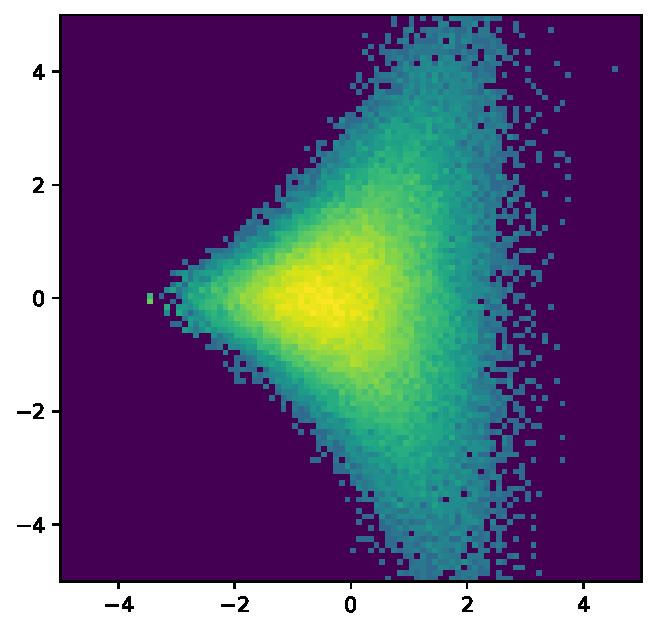
\includegraphics[width=.22\linewidth]{pics/histogram_true_funnel1.pdf}
         &  
          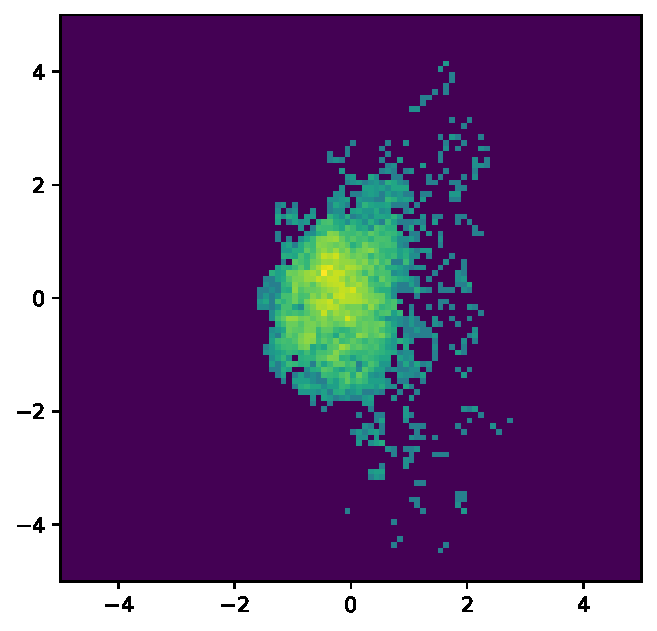
\includegraphics[width=.22\linewidth]{pics/histogram_isir_funnel1.pdf}
          &
           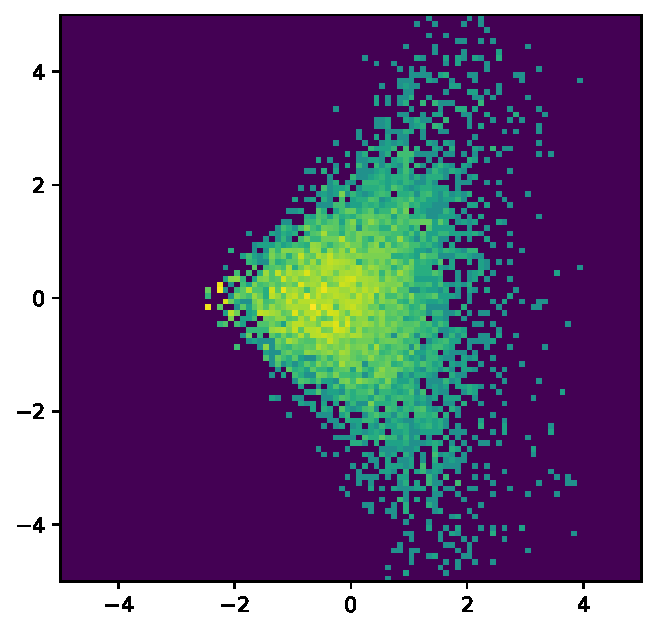
\includegraphics[width=.22\linewidth]{pics/histogram_nuts_funnel1.pdf}
           &
            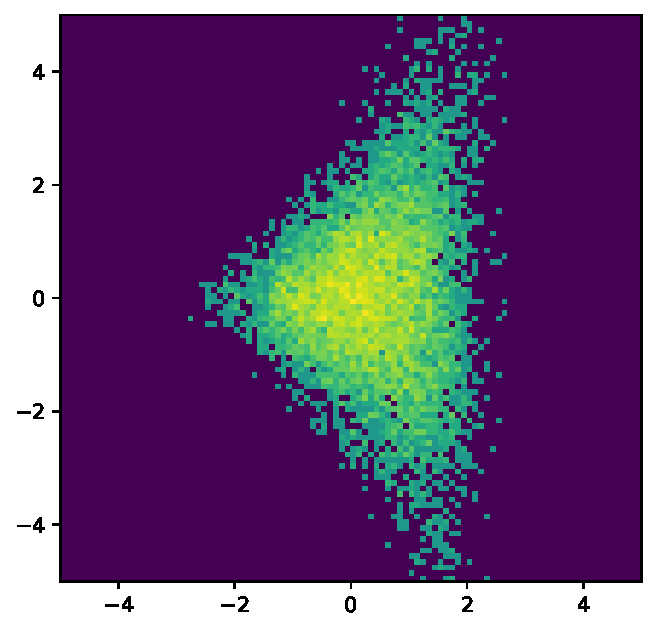
\includegraphics[width=.22\linewidth]{pics/histogram_infine_funnel2.pdf}
    \end{tabular}
\end{figure}
We also present the normalizing constant estimation of this distribution. We initialize the mass matrix and the step-size as discussed previously, and compare IS, AIS, and \InFiNE\ schemes.
The IS estimator is run with $2\cdot 10^5$ samples.
For the \IFIS\ estimator, the number of samples is $N = 2\cdot 10^4$ and the trajectory length is $K=10$. The AIS estimator is run with $2\cdot 10^4$ samples, with the annealing scheme presented in \citep[Section 6.2]{grosse2015sandwiching} of length $K=50$. Moreover, the parameters of the HMC transitions in AIS (mass matrix, step-size) are set to the estimated parameters of the HMC algorithm in Pyro. 
\begin{figure}[!ht]
    \centering
    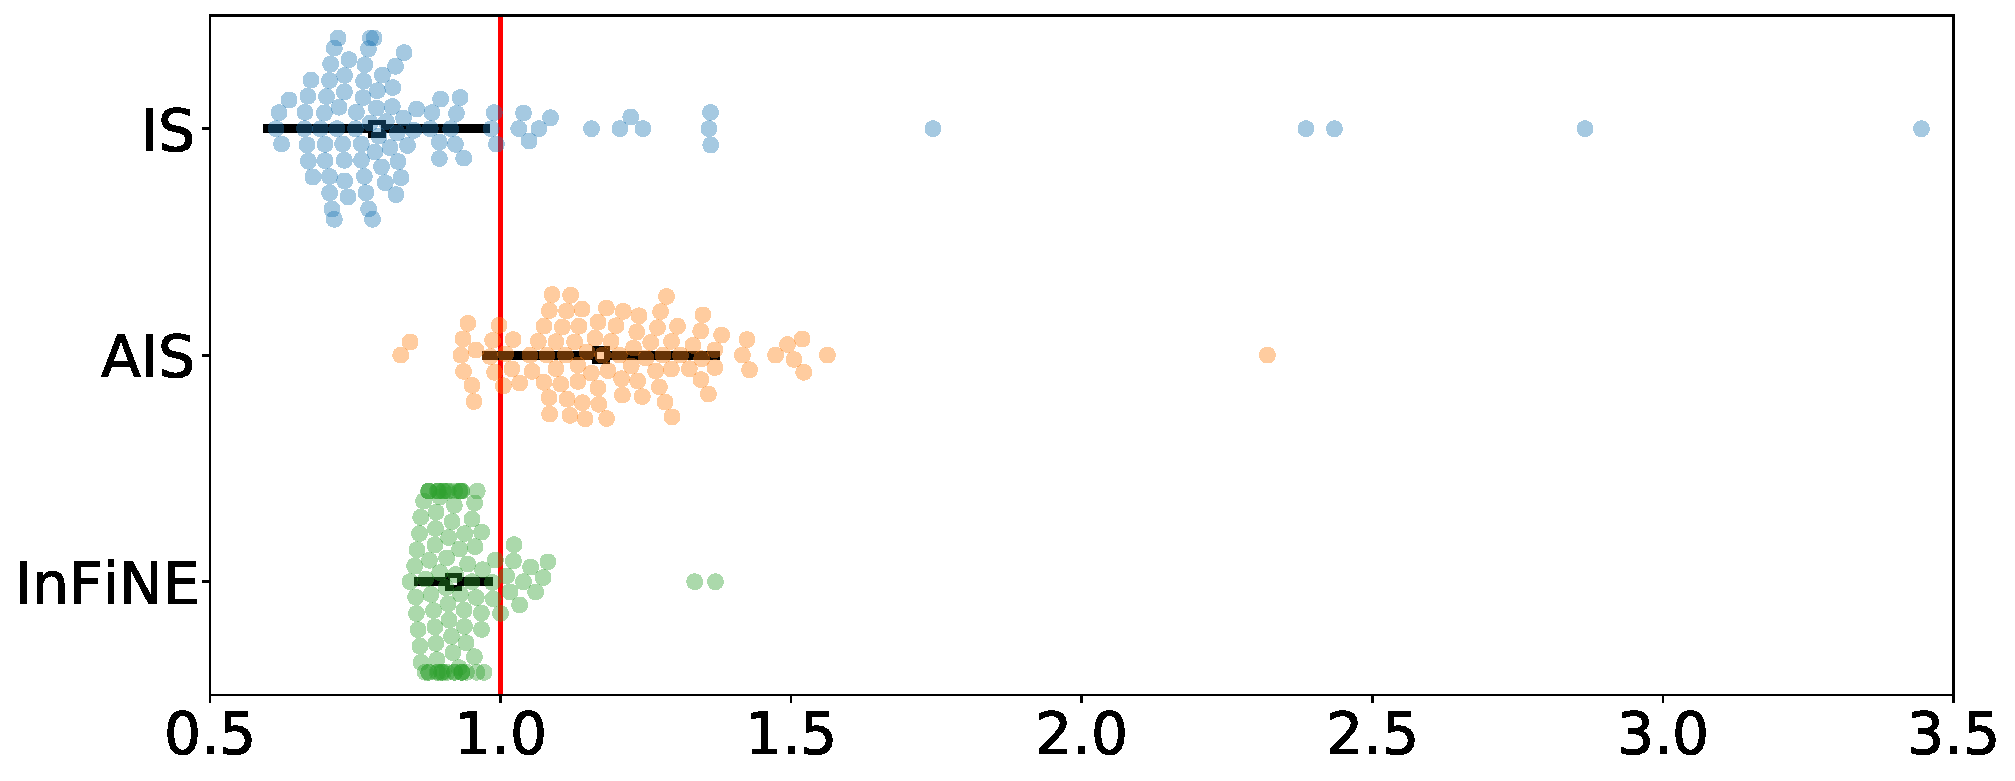
\includegraphics[width=0.7 \linewidth]{pics/funnel.pdf}
    \label{fig:funnel_estimation}
    \caption{200 independent estimations of the normalizing constant of $\pi$. The prior used is a centered Gaussian distribution with $4\mathbf{I}_d$ as covariance matrix. The true value is $Z=1$ (red line). The figure displays the median (square) and the interquartile range (solid lines) in each case.}
\end{figure}

\subsection{VAE experiments}
\label{supsec:vae_exps}
We detail in this section \InFiNE\ VAE with $N$ samples (similarly to the IWAE algorithm). Recall that for each sample,  a trajectory of length $K$ is produced. 
For simplicity, we use $N=1$ in all our experiments to outline \IFIS\ VAE in several experimental settings. It is expected that extension to $N > 1$ will further improve the results.
%Conclusions drawn on the \InFiNE VAE however still hold for the case $N>1$.
Recall that the  lower bound $\elboneq$ is 
\begin{align*}
    \elboneq(\theta, \phi; y) &= \int_{} \proposal_N( \chunku{x}{1}{N})   \log \estConstC{\chunku{x}{1}{N}} \rmd \chunku{x}{1}{N}\eqsp,\\
&= \int_{} \prod_{i=1}^N q_\phi(x^i\mid y)   \log\left( N^{-1}\sum_{i=1}^N\sum_{k=0}^K w_k(x^i) \frac{p_\theta(y, \transfo^k(x^i))}{q_\phi(\transfo^k(x^i)\mid y)}\right)\rmd \chunku{x}{1}{N}\eqsp.
\end{align*}
Assume here that $q_\phi$ is amenable to the reparameterization trick, that is, there exist some diffeomorphism $V_{\phi,y}$ and some fixed pdf $\densgauss$, such that sampling $x\sim q_\phi(\cdot\mid y)$ boils down to sampling $\epsilon\sim\densgauss$ and set $x = V_{\phi,y}(\epsilon)$.
In the particular case where $N=1$, an estimator of the ELBO and of its gradient are given by
\begin{align*}
    &\widehat{\mathcal{L}}_{\IFIS}(\theta, \phi; y) = \log \sum_{k=0}^K w_k(x) \frac{p_\theta(y, \transfo^k(x))}{q_\phi(\transfo^k(x)\mid y)}\eqsp, \eqsp \text{ where } x\sim q_\phi(\cdot\mid y)\eqsp,\\
    &\nabla \widehat{\mathcal{L}}_{\IFIS}(\theta, \phi; y) = \nabla\log \sum_{k=0}^K w_k(V_{\phi,y}(\epsilon)) \frac{p_\theta(y, \transfo^k(V_{\phi,y}(\epsilon)))}{q_\phi(\transfo^k(V_{\phi,y}(\epsilon))\mid y)}\eqsp, \eqsp \text{ where } \epsilon \sim \densgauss\eqsp.
\end{align*}
This is the setting we consider in our experiments. More generally, inspired by the IWAE approach, we can write an estimator of the ELBO and of its gradient as
\begin{align}
\label{eq:gradient_elboneq}
\nonumber
    &\widehat{\mathcal{L}}_{\IFIS} (\theta, \phi; y) = \log\left( N^{-1}\sum_{i=1}^N\sum_{k=0}^K w_k(x^i) \frac{p_\theta(y, \transfo^k(x^i))}{q_\phi(\transfo^k(x^i)\mid y)}\right)\eqsp, \eqsp \text{ where } \chunku{x}{1}{n}\simiid q_\phi(\cdot\mid y)\eqsp,\\
    &\nabla \widehat{\mathcal{L}}_{\IFIS} (\theta, \phi; y) = \sum_{i=1}^N \varpi_i \nabla\log\left( \sum_{k=0}^K w_k(V_{\phi,y}(\epsilon^i)) \frac{p_\theta(y, \transfo^k(V_{\phi,y}(\epsilon^i)))}{q_\phi(\transfo^k(V_{\phi,y}(\epsilon^i))\mid y)}\right)\\
&\hspace{2.6cm}=\sum_{i=1}^N \varpi_i \nabla\log\estConstC{V_{\phi,y}(\epsilon^i)} \eqsp, \eqsp \text{ where } \chunku{\epsilon}{1}{n} \simiid \densgauss\eqsp,
\end{align}
where $\varpi_i = \estConstC{x^i}/(N\estConstC{\chunku{x}{1}{n}})$.
\begin{algorithm}[h]
\label{alg:sup:vae}
\caption{\IFIS\ VAE, trajectory length $K$, and $N$ samples}
\begin{algorithmic}
   \STATE {\bfseries Input:} batch of samples $x$, latent dim $d$.
   \STATE $(\mathbf{\mu}, \log\, \mathbf{\sigma}) \leftarrow EncoderNeuralNet_\phi(x)$.
   \STATE Sample $N$ initial position and momentums: $q_i \sim \mathcal{N}(\mathbf{\mu},\,\operatorname{diag}(\mathbf{\sigma}^{2}))$ and $p_i \sim \mathcal{N}(0, \mathbf{I}_d)$.
   \FOR{$i=1$ {\bfseries to} $N$}
   \STATE Compute $\transfo^k(q_i, p_i)$
   \textit{ This implies forward / backward passes in the decoder to get} $\nabla \log p_\theta(q^k_i)$.
   \STATE Compute $\varpi_i$.
   \ENDFOR
   \STATE Compute the $\ELBO_{\theta, \phi}$ gradient estimator \eqref{eq:gradient_elboneq}.
   \STATE SGD update of parameters $(\theta, \phi)$ using the gradient estimatior.
\end{algorithmic}
\end{algorithm}

\Cref{tab:vae_results} displays the Negative loglikelihood estimates using both IS and \IFIS\ on the FashionMNIST dataset \cite{xiao2017fashion}. The settings are the same than those used in the MNIST experiment. The conclusions are similar:  the \IFIS\ estimate is almost always better than the IS estimate, by a large margin on small dimensions. The InFiNE VAEs are always better than standard VAEs, and better than IWAE with $N=30$ when the dimension of the latent space is small to moderate. When the dimension of the latent space increases ($d=50$), the  performance differences become relatively small.
\begin{table*}[h]
\centering
\caption{NLL estimates for VAE models on FashionMNIST for different latent space dimensions.}
\label{tab:vae_results}
\begin{tabular}{c|c|c||c|c||c|c||c|c|}
\cline{2-9}
 & \multicolumn{2}{c||}{$d = 4$} & \multicolumn{2}{c||}{$d = 8$} & \multicolumn{2}{c||}{$d = 16$} & \multicolumn{2}{c|}{$d = 50$} \\ \hline
\multicolumn{1}{|c|}{model} & IS & \InFiNE  & IS & \InFiNE& IS  & \InFiNE & IS & \InFiNE \\ \hline
\multicolumn{1}{|c|}{VAE} & $240.61$&$240.19$&$235.78$&$235.73$&$235.02$&$234.96$&$234.82$&$234.83$\\ %\hline
\multicolumn{1}{|c|}{IWAE, $N=5$} & $239.66$&$239.27$&$234.05$&$233.98$&$233.12$&$233.12$&$233.52$&$233.46$ \\ %\hline
\multicolumn{1}{|c|}{IWAE, $N=30$} & $239.25$&$238.47$&$233.63$&$233.49$&$233.01$&$232.71$&$232.88$&$232.76$ \\ \hline
\multicolumn{1}{|c|}{\InFiNE\ VAE, $K=3$} & $238.64$&$237.91$&$233.49$&$233.48$&$233.26$&$233.09$&$233.33$&$233.35$ \\ %\hline
\multicolumn{1}{|c|}{\InFiNE\ VAE, $K=10$} & $238.89$&$238.46$&$233.51$&$233.45$&$233.24$&$233.15$&$233.28$&$233.26$ \\ \hline
\end{tabular}
\end{table*}

%\subsection{VAE algorithm}
%\label{subsec:vae_algo}


%Inputs: Select a batch of samples ${x}$
%\begin{enumerate}[wide, labelwidth=!, labelindent=0pt, %label=(\arabic*)]
%\item For $i \in [N]$, compute $\{\transfo^k(X_{n+1}^i)\}_{k=1}^K$
%\item Draw $I_{n+1} \sim %\operatorname{Cat}[(\estConstC{X_{n+1}^{i}})_{i \in [N]}]$
%\item Draw $K_{n+1} \sim \operatorname{Cat}[(\omega_{k,n+1})_{k=0}^K$
%\end{enumerate}




\section{Connection with Nested sampling}

%%%%%\subsection{Computing Normalizing constant}

We return here to the problem of computing the normalizing constant $\const$ of the target density $\pi(x) =\rho(x)\likelihood(x)/\const$ to point out a simplification induced by our method compared to the method proposed in \cite{rotskoff:vanden-eijden:2019}.
The method proposed in \cite{rotskoff:vanden-eijden:2019} uses the identity
\begin{equation}\label{eq:nesting}    \const=\int \int_{0}^{\infty}\1(\likelihood(x)> \ell)\rho(x) \rmd \ell \rmd x =\int_0^\infty \mathbb{P}_{X\sim\rho}(\likelihood(X)> \ell) \rmd \ell\eqsp,
\end{equation}
which was instrumental in the construction of nested sampling
\cite{skilling2006nested,chopin:robert:2010}. Using identical level sets as \cite{skilling2006nested}, of the form $\mso:=\{x:\likelihood(x)>\ell\}$ with $\ell>0$ and their dissipative Langevin dynamics, \citep[Equation 13]{rotskoff:vanden-eijden:2019} obtain a concise estimator of the volume of these level sets based on the length of the path $(\transfo^k(X^i))_{k\in\mathbb N}$ remaining inside $\mso$. (This estimator is constructed under a uniform prior assumption and continuous-time integrator, but the argument in \cite{rotskoff:vanden-eijden:2019} easily translates to discrete-time.)

Considering instead \IFIS, it provides an approximation of $\mathbb{P}_{X\sim\rho}(\likelihood(X)> \ell)$ for
a fixed $\ell$, but a more efficient resolution is available, which bypasses repeated approximations induced by the quadrature version of both \cite{skilling2006nested,rotskoff:vanden-eijden:2019}. The crux of the improvement is that paths only need be simulated once, using only the stopping time associated with the lowest positive $\ell$ found in early simulations. Integration over the likelihood levels $\ell$ can then be accomplished with no further approximation. Using a single stopping time as indicated earlier, the following is an unbiased estimator of $\PP_{X\sim\rho}(\likelihood(X)> \ell)$ for all values of $\ell$: 
\begin{equation}
\widehat{\PP}_{X\sim\rho}(\likelihood(X)> \ell) =\frac{1}{N} \sum_{i=1}^N 
 \sum_{k=0}^K \indiacc{\likelihood(\transfo^{k}(X^i))> \ell} \w_k(X^i)\eqsp,
 \qquad
X^{i}\stackrel{\text{iid}}{\sim}\rho\eqsp,
\end{equation}
where the weights $\w_k(X^i)$, defined in \eqref{eq:w_k_first_def}, incorporate the stopping times. Integrating the above over $\ell\in\mathbb{R}^+$ as in \eqref{eq:nesting} leads to an estimator of the normalizing constant $\const$:
\begin{align}\label{eq:nolevel}
\widehat{\const}_{X^{1:N}} &=\frac{1}{N}\sum_{i=1}^{N} \sum_{k=0}^{K}  \int_{\mathbb{R}^+} 
 \mathbb{I}(\likelihood(\transfo^{k}(X^i))> \ell) \w_k(X^i) \rmd \ell\nonumber\\
 &= \frac{1}{N}\sum_{i=1}^{N} 
 \sum_{k=0}^K\likelihood(\transfo^k(X^i)) \w_k(x^i)\eqsp,
\end{align}
where we used the slice sampling identity 
\[ 
 \int_{\mathbb{R}^+} \indiacc{\likelihood(\transfo^{k}(x))> \ell} \rmd \ell=\likelihood(\transfo^{k}(x))\eqsp.
\]
In conclusion, the \IFIS~estimator of $\const$ coincides with the conformal Hamiltonian version of nested sampling with the additional benefit of removing the quadrature approximation.
(Note that, as suggested \Cref{remark1}, we could resort to both forward and backward push-forward rather than starting at $k=0$, which could only improve the precision of the estimator \eqref{eq:nolevel}.)


\begin{comment}
\subsection{Approximate sampling from the target}
We have
\begin{align*}
    \int_\Omega \dummy(x) \rho(x) L(x) \rmd x&= \int_{L_{\min}}^{L_{\max}} \int_\Omega  \dummy(x) \rho(x) \delta_{\{x:L(x)=L\}}(\rmd x)~L \rmd L\\
    &=  \int_{\rset^+} \frac{\int_\Omega \dummy (x) \rho(x) \delta_{\{x:L(x)=L\}}(\rmd x)}{\int_\Omega \rho(x) \delta_{\{x:L(x)=L\}}(\rmd x)}    \int_\Omega \rho(x) \delta_{\{x:L(x)=L\}}(\rmd x)~L \rmd L\\
    &=  \int_{\rset^+} \int_\Omega \dummy(x) \eta_L(\rmd x) \int_\Omega \rho(x) \delta_{\{x:L(x)=L\}}(\rmd x)~L \rmd L,
\end{align*}
where $\eta_L$ is the probability measure on the level set $\{x:L(x)=L\}$ defined by 
\begin{align*}
    \int_\Omega \dummy(x) \eta_L(\rmd x)&= \frac{\int_\Omega \dummy (x) \rho(x) \delta_{\{x:L(x)=L\}}(\rmd x)}{\int_\Omega \rho(x) \delta_{\{x:L(x)=L\}}(\rmd x)},
\end{align*}
and the derivative $V'(L)$ of $V(L)$ w.r.t. $L$ is 
$V'(L)=-\int_\Omega \rho(x) \delta_{\{x:L(x)=L\}}(\rmd x)$. Note that notations are not consistent in \cite{rotskoff:vanden-eijden:2019} as $V(L)$ is decreasing w.r.t. $L$ whereas in the previous section $V(E)$ is increasing w.r.t. $E$.
We also have
\begin{align*}
 Z=\int_\Omega \rho(x) L(x) \rmd x&=\int_{\rset^+} V(L)\rmd L\\
                                 &=- \int_{\rset^+} L V'(L)\rmd L.
\end{align*}
So overall, we have
\begin{align*}
    \int_\Omega \dummy(x) \pi(x) \rmd x&=\frac{\int_{\rset^+} \int_\Omega \dummy(x) \eta_L(\rmd x)~ V'(L)L \rmd L}{\int_{\rset^+} V'(L)L \rmd L}\\
    &=-\frac{\int_{\rset^+} \int_\Omega \dummy(x) \eta_L(\rmd x)~ V'(L)L \rmd L}{\int_{\rset^+} V(L) \rmd L}
\end{align*}

Hence we can can sample from $\pi$ by first sampling $L \sim \lambda(\cdot)$ where $\lambda(L)\propto V'(L)L$ then $X\sim \eta_L(\cdot)$. 

This suggests that to sample 
approximately from $\pi$ using the algorithm output, we can sample from 
\begin{align*}
    \hat{\lambda}(\rmd L) \propto \sum_{i=1}^N \frac{\sum_{k=\tau_{T}^{-}( X^i)+1}^{\tau_{T}^{+}( X^i)-1} \rho\left(\phi^{k}( X^i)\right)|\Jac{\phi^{k}}( X^i)|L(\phi^{k}( X^i)) \delta_{L(\phi^{k}( X^i))}(\rmd L)}{ \sum_{j=\tau_{T}^-( X^i)+1}^{\tau_{T}^+( X^i)-1}  \rho(\phi^{j}( X^i)) |\Jac{\phi^{j}}( X^i)|}
\end{align*}
and sampling $X\sim \hat{\eta}_{L}$ corresponds to setting $X=\phi^k(X^i)$ such that $L=L(\phi^{k}( X^i))$ (under mild assumptions this point is unique). So by combining both 
kernels, we simply obtain
\begin{align*}
    \hat{\pi}_{X^{1:N}}(\rmd x) \propto \sum_{i=1}^N \frac{\sum_{k=\tau_{T}^{-}( X^i)+1}^{\tau_{T}^{+}( X^i)-1} \rho\left(\phi^{k}( X^i)\right)|\Jac{\phi^{k}}( X^i)|L(\phi^{k}( X^i)) \delta_{\phi^{k}( X^i)}(\rmd x)}{ \sum_{j=\tau_{T}^-( X^i)+1}^{\tau_{T}^+( X^i)-1}  \rho(\phi^{j}( X^i)) |\Jac{\phi^{j}}( X^i)|}
\end{align*}
\end{comment}
\bibliography{bibliography}
\bibliographystyle{icml2021}

\end{document}


